% This document provides the style to be used for a MSc Thesis at the
% Parallel and Distributed Systems group
\documentclass[11pt,twoside,a4paper,openright]{report}

% math packages
\usepackage{amsthm}
\usepackage[fleqn]{amsmath}
\usepackage{amssymb}

%\usepackage{subfig}
 \usepackage{floatrow}
\usepackage{algorithmicx}
\usepackage{algorithm}
\usepackage{algpseudocode}
\usepackage[toc,page]{appendix}
\usepackage{caption}
\usepackage{subcaption}
\usepackage{graphicx,wrapfig,lipsum}


% textblocks for title page
\usepackage[absolute]{textpos}
\usepackage{tikz}

% use babel for proper hyphenation
\usepackage[british]{babel}
\bibliographystyle{./bib/myCustom}
%\bibliographystyle{abbrvnat}
\usepackage[numbers,sort&compress]{natbib}
\usepackage{bytefield}

% Graphics: different for pdflatex or dvi output, choose one
%%\usepackage[dvips]{graphicx}
%%\usepackage[pdftex]{graphicx}
\usepackage{graphicx}

\usepackage{epstopdf}
\usepackage{rotating}


% FONT
\usepackage[scaled=.92]{helvet}
%\usepackage{times}

% for url's use "\url{http://www.google.com/}"
\usepackage{url}
\usepackage{hyperref}

\hypersetup{
  colorlinks   = true, %Colours links instead of ugly boxes
  urlcolor     = cyan, %Colour for external hyperlinks
  linkcolor    = cyan, %Colour of internal links
  citecolor   = cyan %Colour of citations
}
\usetikzlibrary{shapes,arrows,graphs,positioning,automata,shadows,fit,shapes,decorations.pathreplacing}
\tikzset{
    rotate around with nodes/.style args={#1:#2}{
        rotate around={#1:#2},
        set node rotation={#1},
    },
    rotate with/.style={rotate=\qrrNodeRotation},
    set node rotation/.store in=\qrrNodeRotation,
}
\usepackage{etoolbox}
\appto\appendix{\addtocontents{toc}{\protect\setcounter{tocdepth}{0}}}

% reinstate the correct level for list of tables and figures
\appto\listoffigures{\addtocontents{lof}{\protect\setcounter{tocdepth}{1}}}
\appto\listoftables{\addtocontents{lot}{\protect\setcounter{tocdepth}{1}}}

\def\algbackskip{\hskip\dimexpr-\algorithmicindent+\labelsep}
\def\LState{\State \algbackskip}%
% Information that will be filled in at various points in the report
\newcommand{\reportTitle}{TODO TITLE}
\newcommand{\reportAuthor}{Arpan Govindraju}
\newcommand{\reportEmail}{a.govindaraju@student.tudelft.nl}
\newcommand{\reportUrlEmail}{\href{mailto:\reportEmail}{\reportEmail}}
\newcommand{\reportMSC}{MSc Embedded Systems} %{Embedded Systems}{Computer Engineering}{Computer Science}{Electrical Engineering}
\newcommand{\reportDate}{\today} %TODO: Dit is de datum van uitgifte van final versie aan de afstudeer commissie 
\newcommand{\presentationDate}{\today} %TODO: Dit is de datum van de afstudeerpresentatie 
\newcommand{\graduationCommittee}{
TODO GRADUATION COMMITTEE & Delft University of Technology \\
TODO GRADUATION COMMITTEE & Delft University of Technology \\
} % The order of listing the names: Graduation prof, supervisor(s), others ordered by title + alphabetical 
%examples: 
%prof. dr. ir. H. J. Sips (chair) & Delft University of Technology \\ 
%ir. dr. D. H. J. Epema           & Delft University of Technology \\ 
\newcommand{\reportAbstract}{TODO ABSTRACT}
\newcommand{\reportKeywords}{TODO KEYWORDS}
%\newtheorem{theorem}{Theorem}[section]
\theoremstyle{definition}
\newtheorem{definition}{Definition}[section]


% For pdflatex
\pdfinfo{
   /Author (\reportAuthor)
   /Title  (\reportTitle)
   /Keywords (\reportKeywords)
}

\begin{document}

\pagenumbering{alph}
\pagestyle{empty}


% FRONTCOVER
\include{frontcover}

%%%%%%%%%%%%%%%%%%%%%%%%%%%%%%%%%%%%%%%%%%%%%%%%%%%%%%%%%%%%%%%%%%%%%%%%%%%%%%%
\hoffset=1.63cm
\oddsidemargin=0in
\evensidemargin=0in
\textwidth=5in

%%%%%%%%%%%%%%%%%%%%%%%%%%%%%%%%%%%%%%%%%%%%%%%%%%%%%%%%%%%%%%%%%%%%%%%%%%%%%%%
\parindent=1em

% EMPTY PAGE
\cleardoublepage

\pagestyle{plain}
\pagenumbering{roman}
\setcounter{page}{1}

% TITLE PAGE: page i (hidden)
\include{titlepage}

% GRADUATION DATA AND ABSTRACT: pages ii and iii (hidden)
\include{./template/graduationdata}
%\setcounter{page}{4}

% EMPTY PAGE: page iv
\cleardoublepage

% OPTIONAL QUOTATION: page v
%\pagestyle{empty}

\null\vfill

\begin{center}
\emph{`Location, Location, Location''} -- Harold Samuel
\end{center}

\vspace{10cm}

\clearpage


% EMPTY PAGE: page vi
%\cleardoublepage

% PREFACE: page v
\chapter*{Preface}
\addcontentsline{toc}{chapter}{Preface}


\vspace{1\baselineskip}

\noindent
Indoor spaces are getting smarter day by day with deployment of huge amount of sensors and actuators. Many applications built for maintenance of the building use the sensor data as inputs to actuate the actuators to perform their function. May it be simple turning on and off of lights based on occupancy or a more critical applications like fire detection and alarming, all need data from the sensors. One important meta-data about the sensor, that is crucial for all theses application is the sensor location. Without which the applications cannot perform effectively. Till now the meta-data is being created and maintained manually, which is a cumbersome process and prone to error. In our work here we propose a method to automatically determine the location of the sensor using the data from the sensors.

This work was carried out at Philips Lighting, Eindhoven. Philips Lighting being a market leader in the field of lighting are actively providing lighting control solutions. This work is aimed to help automate the process of creating and maintaining the meta-data of sensor location and thus aiding faster deployment and easier maintenance of the systems.

Before going to the technical details of the thesis, I would like to thank my supervisor Dr.Ashish Pandharipande(Philips Lighting) for giving me an opportunity to carry out my thesis at Philips Lighting. I would also like to thank him and Dr.David Caicedo Fernandez(Philips Lighting) for critically analyzing my work during our regular weekly meetings and giving me valuable suggestions. My sincere gratitude to my university supervisor Dr.Venkatesh Prasad(TU Delft) for all the support and guidance he provided. I would also like to thank my parents and grandparents for their unconditional love and support during all these years.
I would like to thank all my friends who have tolerated my constant whining and supported me during my tough times.
A special thanks to all the people of FO 52, past and the present who made the stay in Eindhoven so much more pleasant.

\vspace{1\baselineskip}

\noindent
Arpan Goindaraju\\
%\vspace{1\baselineskip}
%\noindent
Eindhoven, The Netherlands\\
%\noindent
\today

% EMPTY PAGE: page vi
\cleardoublepage

% TABLE OF CONTENTS: starting at page vii
\tableofcontents
%S\setcounter{tocdepth}{1}

\cleardoublepage

\pagenumbering{arabic}
\setcounter{page}{1}

% INTRODUCTION: page 1
\chapter{Introduction}
\label{chp:introduction}
\section{Motivation}
The European Union (EU) has pledged to cut the consumption of primary energy by 20\%, by the year 2020.  It is estimated that buildings consume 40\% of the energy produced\footnote{according to value published at https://ec.europa.eu/energy/en/topics/energy-efficiency/buildings }.  This has resulted in an increase in the demand to reduce the energy consumption of buildings. To reduce the consumption of energy, building automation systems (BAS) are being widely employed. BAS are computer-based systems that help to manage, control and monitor building technical services (HVAC, lighting etc.) and the energy consumption of devices used by the building. It is estimated that BAS can save a building between 5 percent to 30 percent on the utility cost by managing HVAC and lighting systems\cite{bas}.

BAS deploy a huge amount of sensors, which provide inputs to perform efficient control of various services. BAS brings with it various benefits, at the same time, offers numerous challenges too. For BAS, sensor measurements alone are not sufficient to understand the condition of the facilities, unless combined with meta-data associated with the sensors.
Meta-data as defined in \cite{gao2015data} refers to any information associated  with the device that helps to contextualize the measurements or control signals regularly being sent from/to the device, such as the location within the building, the physical phenomenon being sensed, etc. One of the major challenges in a BAS system is generating and updating the meta-data of the sensor.
One of the important meta-data required is that of the physical location of the sensor as discussed in  \cite{liu2009requirements}.
As the size and distribution of the deployed sensors are high, it is highly cumbersome and error prone to manually maintain the meta-data about the sensor placement. Apart from being error prone, the manual configuration has to be repeated every time there is a change in the meta-data. Change in meta-data can be due to various reasons, such as a change in the office setup, replacement and/or relocation of sensors. All these factors result in inaccurate information about the location of the sensors. Without the accurate information of the location of the sensors, interpreting the data collected from the sensor is difficult and also can be misleading. This could result in the decrease in the effectiveness of the deployed BAS systems. Hence there is a need to develop methods to accurately determine the location of the sensors within the building.
\section{System Description}
Smart lighting control is one of the major components of BAS. Lighting is responsible for 11 percent  and 18 percent of the energy consumption in case of residential and commercial buildings respectively\cite{website}. 
State of the art lighting control employs co-located occupancy sensors and light sensors, placed on luminaries which are attached to the ceiling\cite{pandharipande2015smart,caicedo2016smart,van2014distributed}.
In this thesis, we consider such ceiling based sensor grid consisting of occupancy sensors. We represent the sensor grid as a graph $G$ with the sensors located on the vertices of the graph.

\section{Problem Statement}

Several studies \cite{Hong:2013:TAS:2528282.2528302,doi:10.1061/9780784413616.226,Koc:2014:CLC:2674061.2674075,Lu:2014:SBS:2648771.2629441,ellis2012creating,muller2014automated,marinakis2005learning} have been carried out to infer the sensor location from sensor data. Most of the methods developed so far have identified ways to cluster the sensors that are located within their proximity; however the methods do not identify where exactly on the grid each sensor is located in a dense sensor grid \cite{Hong:2013:TAS:2528282.2528302,doi:10.1061/9780784413616.226,Koc:2014:CLC:2674061.2674075}.  Therefore the research question that is being tackled in this work is:

\textit{How to Automatically determine the location of the sensors utilizing binary data from the ceiling mounted occupancy sensors and the information about the grid (coordinates of the vertices constituting the grid)?}

\section{Contribution of the thesis}
The main contribution of the thesis are:
\begin{itemize}
\item Energy feature of the binary occupancy sensor data is used to distinguish between neighboring and non neighboring nodes.
\item Reducing the problem of determination of sensor locations  on the grid to a problem of graph matching \cite{conte2004thirty}.
\end{itemize}

\section{Outline of thesis}

The rest of the thesis is organized as follows: in chapter 2, we give a brief overview of related work. In chapter 3, we present the method that has been developed. In chapter 4, we describe our testbed setup. Next, in chapter 5, we present the results obtained by applying the method that we have developed on actual sensor data obtained from 2 different testbeds. In the end in chapter 6, we conclude the work done and discuss future work.


%\section{Application}
%FOr few of the applications like the one developed in 




\vspace{1\baselineskip}

\noindent
%TODO ORGANISATIONAL DESCRIPTION OF THESIS





% CHAPTERS ... For instance: History/Prior Work, Design/Implementation, Experiments
\chapter{Literature Review}
\label{chp:litReview}
\section{Sensor Localization}
There has been an extensive body of research that aims at obtaining the location information of the sensors in wireless sensor networks (WSN). All the approach that has been taken till now has been categorized by \citeauthor{wang2010survey} in \cite{wang2010survey} to fall into one of the following categories:
\begin{itemize}
\item Proximity based localization
\item Range based localization
\item Angle based localization
\end{itemize}

In \textbf{\textit{proximity based localization}} \cite{bulusu2000gps,4317866,shang2003localization}, WSN is represented as a graph $G(V,E)$. $V$ representing the location of the sensor nodes, $E$ representing the connectivity between two nodes which are within each others proximity. Location of the  subset of the nodes, $H \subset V$ called as anchor nodes are known. The goal is to estimate the location of the remaining non anchor nodes relative to the position of the anchor nodes. 

\textbf{\textit{Range based localization}} makes use of  ranging techniques using RSSI \cite{mao2007path}, time of arrival (ToA) \cite{moses2003self} and time difference of arrival (TDoA) of the signals \cite{4058681}. The distance between the nodes is computed using the ranging technique. Computing the locations of the nodes using distance information is non trivial. Range based approach may or may not need anchor nodes. With anchor based approach multilateration technique is used to find the location of the non anchor nodes. Without anchor nodes, multi dimensional scaling (MDS) is adopted for localization. 

\textbf{\textit{Angle based  localization}} uses the information of angle of arrival (AoA) of the signals to determine the location of the sensors \cite{nasipuri2002directionality,rong2006angle}. To determine the angle, antenna array or multiple receivers on the node are required.

In the case of proximity based localization, the locations of the anchor nodes are required to compute the locations of the remaining nodes, which might not be available always. The major drawback for the range based and angle based algorithm is that the nodes require specialized hardware to measure ToA/TDoA, AoA \cite{4317866} thereby, increasing the cost per sensor node. As BAS employs a large number of sensors, using such specialized hardware becomes infeasible as the total cost of the system increases. Calculating distance based on the RSSI is prone to noise of the order of several meters \cite{bachrach2005localization}, as the propagation of radio waves is non uniform in an indoor environment.

\subsection{Data driven sensor localization}

Data driven sensor localization has gained attention recently. The main advantage of this approach is that it does not require any special hardware, extra processing power on the nodes or extra information like RSSI to perform the localization.
It makes use of the sensor data collected for the functioning of the applications deploying the sensors. 
As our work falls under the same category, we provide an overview of related works using the sensor data to determine the sensor location. For convenience we categories the works in this area to the following categories:
\subsubsection*{Sensor Localization in Commercial Buildings}
The works presented below consider a system set up in commercial buildings.
 In \cite{Hong:2013:TAS:2528282.2528302}, \citeauthor{Hong:2013:TAS:2528282.2528302} 
 apply empirical mode decomposition (EMD) to 15 sensors in 5 rooms to cluster sensors which belong to the same room by analyzing the correlation coefficients of the intrinsic mode functions (IMF). They characterize the correlation coefficient distribution of sensors that are located in the
 same room and different rooms. They were able to show that there exists a correlation boundary analogous to the physical boundary which can be discovered empirically. 
In \cite{doi:10.1061/9780784413616.226}, \citeauthor{doi:10.1061/9780784413616.226} propose a feature: energy content in HVAC delivered air, which can be derived from HVAC system sensors which could lead to the identification of the space in which the sensors are located . They combine sensor measurements and building characteristics(floor area) for the identification of the space in which the sensors are present.
In \cite{Koc:2014:CLC:2674061.2674075}, \citeauthor{Koc:2014:CLC:2674061.2674075} propose a method to automatically identify the zone temperature and discharge temperature sensors that are closest to each other by using a statistical method on the collected raw data. They explore whether linear correlation or a statistical dependency measure(distance correlation) are better suited to infer the spatial relationship between the sensors. They carry out their analysis on three different testbeds. They also investigate the effects of distance between sensors and measurement periods on the matching results. In the end, the authors conclude that linear correlation coefficient provides better matching results compared to distance correlation. The authors also conclude that as the distance between the sensors increase, the data size needed to infer spatial relationships also increase.
\subsubsection*{Sensor Localization in Smart homes}
The works presented below, consider a system set up in smart homes. 
\citeauthor{Lu:2014:SBS:2648771.2629441} \cite{Lu:2014:SBS:2648771.2629441} describe a method to generate representative floor plans for a house. Their method clusters sensors to a room and assigns connectivity based on the simultaneous firing of the sensors placed on the door and window jambs. The algorithm gives a small set of possible maps from which the user has to choose the right map. Method requires special placement of the sensors to eliminate false clusters caused due to simultaneous occupancy of multiple rooms. The authors were able to calculate the floor map of 3 out of the 4 houses they evaluated.  
 \citeauthor{ellis2012creating} \cite{ellis2012creating} proposed an algorithm to compute the room connectivity using  PIR and light sensor data. They cluster the sensors present in the same room based  on observing the simultaneous triggering of the sensors. After clustering, they compute room connectivity based on, the artificial light spill over between rooms; occupancy detection due to movements between
  rooms; and fusion of the two. They calculate the transition matrix for the light sensor and occupancy sensor. Fuse both the data together to compute the connectivity graph. Here the authors have considered a situation where there are only one PIR and light sensor per room.
\citeauthor{muller2014automated} \cite{muller2014automated} define  sensor topology as a graph with directed and weighted edges. All pairs of consecutive sensors triggers are interpreted as a user walking from the former to the latter sensing region indicated in the sensor 
graph by an edge from the former to the latter. Every time a consecutive edge triggers are observed the weight of the edge between the sensors is incremented. They define a method to filter out erroneous edges.
\subsubsection*{Sensor Localization by activity recognition}
In \cite{marinakis2005learning}, \citeauthor{marinakis2005learning} obtain the sensor network topology using Monte Carlo Expectation Maximization. They assign activity to people present in the space to obtain the graph topology. The algorithm requires, the number of people present in the space as the input. They demonstrate the effectiveness of the algorithm using various simulated data.
\subsubsection*{Limitations}
The methods presented in \cite{Hong:2013:TAS:2528282.2528302,doi:10.1061/9780784413616.226,Koc:2014:CLC:2674061.2674075,muller2014automated} look at only clustering the neighboring sensors together. They do not provide the information about where the sensors are located in the sensor grid. \cite{ellis2012creating,Lu:2014:SBS:2648771.2629441,muller2014automated} consider a smart home setting where sensors are sparsely located to identify their positions. Method proposed in \cite{Lu:2014:SBS:2648771.2629441} requires special placement of sensors in the room to aid them in locating the sensors. In \cite{ellis2012creating}, the authors assume that there is only one sensor per room which makes it not applicable to systems which employ more than one sensor in a room. 

The method we propose is able to locate the sensor on the grid. Our approach does not limit the number of sensors present with in a room nor does it require any special placement of sensors. The only condition that we apply is that a sensor should have an overlapping field of view with other sensors.


\section{Meta-data inference}

As explained in section \ref{sec:motivation}, there is a need to automate the process of determining meta-data information of sensors. Due to which there has been significant interest shown to develop such methods. The works in this area can be classified in to two categories: inference from tags and inference from data
\subsection{Inference from Tags}
In general meta-data of the sensors are embedded in the tags that are given to the sensors. These tag names are highly unstructured and inconsistent as different tags are added by different installers. HVAC systems might be installed by a certain company, whereas lighting controls are installed by another company. These installers tag the sensors and actuators based on their own conventions and convenience. Though there has been significant efforts to standardize the convention of naming the tags, no solution has been widely accepted \cite{gao2015data}. Hence there have been methods developed to infer the meta-data automatically from these unstructured tags.

In \cite{bhattacharya2014enabling}, \citeauthor{bhattacharya2014enabling} developed a technique to convert the tags of the sensors to a common and understandable name space. The method learns from a small number of example of the tags, which is provided by an expert, such as the building manager. From this representative examples, the method deciphers the rest of the tags of the sensors that are part of the system.
In \cite{Schumann:2014:TAD:2674061.2674081}, \citeauthor{Schumann:2014:TAD:2674061.2674081} use the semantics of the textual labels of the sensor tags for semi-automating the process of inferring the meta data associated with sensors.
\subsection{Inference from Data}
Works \cite{Hong:2013:TAS:2528282.2528302,doi:10.1061/9780784413616.226,Koc:2014:CLC:2674061.2674075,Lu:2014:SBS:2648771.2629441,ellis2012creating,muller2014automated,marinakis2005learning} that were discussed previously fall under this category of inference of meta-data from the sensor measurements. They provide the information about the location of the sensor within the facility. 
Apart from the inference of location of the sensors, there have been few works which derive the information about the sensor type from the data. In \cite{calbimonte2012deriving}, \citeauthor{calbimonte2012deriving} observe the similarity in the slopes of the piece wise linear representation of the raw time-series measurements. Sensors which show similar slopes are categorized as of the same type. In \cite{gao2015data}, \citeauthor{gao2015data} extract statistical features from the data stream and train various classifiers to identify the sensor type.
\section{Graph Matching}
\label{sec:graphLitReview}
We use graph matching technique in our work to determine the location of the sensor on the grid vertices. Depending on the mapping type between the base graph and the pattern graph, graph matching can be categorized into different types. Our problem falls into the category of graph monomorphism. In this section, we present the related works in the area of graph matching in particular we look at works which solve graph monomorphism.

Graph matching is widely used in pattern recognition and image processing applications. Graph matching also finds its application in the field of biomedical and biological applications. 
Most of the algorithms that are developed for the purpose of graph matching employs tree search to iterate through all the nodes when an unfruitful match is encountered the algorithm backtracks.
The key principle is that there will be a partial mapping which will be initially empty and the mappings gets expanded iteratively by adding to it new pairs of matched node. The matched nodes are chosen based on the conditions determined by the matching type.

The first prominent and one of the most widely used algorithm till date in the area of graph matching was proposed by \citeauthor{Ullmann:1976:ASI:321921.321925} \cite{Ullmann:1976:ASI:321921.321925}.
Ullmann algorithm addresses the problem of graph isomorphism, sub graph isomorphism, graph monomorphism. Ullmann algorithm is based on  depth-first search with backtracking.
The author employs a procedure called \textit{refinement procedure}, which prunes unfruitful matches based on the knowledge of the adjacent nodes and the degree of the nodes that are being matched.
\citeauthor{4308468} in \cite{4308468}, proposed a graph monomorphism algorithm.
The authors formulate the graph monomorphism problem as a minimum weight clique problem of weighted nets .
The major drawback of the algorithm is that the algorithm uses a $N^2 \times N^2$ matrix to represent netgraph obtained from the cartesian product of the nodes of two graphs under investigation.
N representing the number of nodes of the largest graph. This leads to large memory consumption, making the algorithm viable for only small graphs.
A more recent algorithm for graph isomorphism, subgraph isomorphism, and monomorphism was proposed by \citeauthor{906251} in \cite{906251}, popular as VF algorithm. 
The authors define a set of rules that are based on the sets of nodes connected to the ones that are already mapped.
The authors further improved the algorithm in 2001 in their paper \cite{cordella2001improved}. 
The authors proposed a modification to the algorithm and called it VF2.
The authors introduce a method to restore data structure, which enabled them to reduce the memory consumption from $O(N^2)$ to $O(N)$ where $N$ is the number of nodes in the graph, thus enabling the algorithm to work with large graphs.

\section{Summary}
In this chapter we give a brief overview of the related work in the field of data driven sensor localization in buildings and meta-data inference technique. We also discuss works related to graph matching technique, which we use in our method to map the sensors to their locations on the grid. Table \ref{tab:litReview} summarizes the data driven localization techniques that have been discussed in this chapter.
Previous data driven methods as discussed in this chapters have successfully clustered co-located sensors using various approaches. But they do not provide any information about the sensors location with respect to the entire sensor grid. We in our work address this issue and propose a technique to identify the location of the sensors on the sensor grid.

\begin{table}[!ht]
\centering
\caption{Summary of data driven localization techniques}
\label{tab:litReview}
\begin{tabularx}{\textwidth}{|X|X|X|}
\hline
Work                                                                               & Purpose                                                                                                     & Method                                                                                                                                                                                                                              \\ \hline
\centering\text{\citeauthor{Hong:2013:TAS:2528282.2528302}}\text{\cite{Hong:2013:TAS:2528282.2528302}} & co-locating sensors                                                                                         & Correlation coefficient between the IMF of the sensor data \\ \hline
\centering\text{\citeauthor{doi:10.1061/9780784413616.226}}\text{\cite{doi:10.1061/9780784413616.226}} & co-locating sensors                                                                                         & Correlation coefficient between the energy content of the HVAC delivered air \\ \hline
\centering\text{\citeauthor{Koc:2014:CLC:2674061.2674075}}\text{\cite{Koc:2014:CLC:2674061.2674075}}      & co-locating sensors                                                                                         & Correlation between the raw sensor data.                                                                                                                                                                                            \\ \hline
\centering\text{\citeauthor{Lu:2014:SBS:2648771.2629441}}\text{\cite{Lu:2014:SBS:2648771.2629441}}      & floor maps for a house                                                                                      & Clustering based on simultaneous trigger of occupancy sensors. Connectivity between rooms is determined by  simultaneous triggering of sensors placed on window jamb and door. \\ \hline
\centering\text{\citeauthor{ellis2012creating}}\text{\cite{ellis2012creating}}                         & room connectivity graph                                                                                     & Transition matrix between the sensors located in different rooms.                                                                                                                                                                   \\ \hline
\centering\text{\citeauthor{muller2014automated}}\text{\cite{muller2014automated}}                     & co-locating sensors                                                                                         & Consecutive edge triggers                                                                                                                                                                                                           \\ \hline
\centering\text{\citeauthor{marinakis2005learning}}\text{\cite{marinakis2005learning}}                  & inferring sensor network topology by assigning activity to users. &Assigning activity to people to obtain the sensor topology                                                                                                                                            \\ \hline
\end{tabularx}
\end{table}




% CONCLUSIONS AND FUTURE WORK
\chapter{Methodology}

This chapter explains the method developed to locate the sensors in a sensor grid, using the information about the locations of the vertices of the grid and data obtained from the sensors. Before we explain the method we introduce the definitions of the terms that 
we use in our thesis.\\
\begin{definition}{Neighboring sensors:}
 Two sensors are said to be neighbors if they have overlapping field of view.
\label{def:ns}
\end{definition}
\begin{definition}{Grid Adjacency Matrix:}
 We represent the sensor grid in the form of an adjacency matrix. Two vertices of the grid i and j are adjacent if the distance between them ($d_{i,j}$) is less than twice the radius(r) of the sensors field of view.

\[
GAM_{i,j} = 
\begin{cases}
1, &\text{ if } d_{i,j} < \text{  2r } \forall \text{ } i \ne j\\
0, & \text{otherwise}\\
\end{cases}
	\]
$d_{i,j}$  is the euclidean distance between the vertex i($x_i$,$y_i$) and j($y_j$,$y_j$).
\begin{equation*}
d_{i,j}=\sqrt{(x_i-x_j)^2 + (x_j-y_j)^2}
\end{equation*}
\label{def:GAM}
\end{definition}
From the definitions \ref{def:GAM} and \ref{def:ns} we can say that neighboring sensors will always be placed on neighboring vertices. 
\section{Feature}
Consider a m $\times$ n grid as shown in the figure \ref{fig:Grid}. There are $N= (m\times n)!$ ways in which the sensors can be uniquely placed on the grid. Out of these N ways we have to identify the actual arrangement of the sensors in the grid.  Along with the information of the vertex locations we also have the data from the sensors available. Using the sensor data along with information available about the grid we develop a method to identify the sensor lcoation of the grid\\
As neighboring sensors have an overlapping field of view, they observe the same events and thus are highly correlated.
On the raw signals of the PIR data stream we use a sliding window with 50\% overlap between the consecutive windows and compute the energy feature using the equation \ref{eq:energyEq}

\begin{equation}
\label{eq:energyEq}
E_s = {\sum_{n=0}^{k}{|x(n)|}^2}
\end{equation}
For a PIR binary data computing energy reduces to counting the number of triggers observed within the window.

\begin{figure}
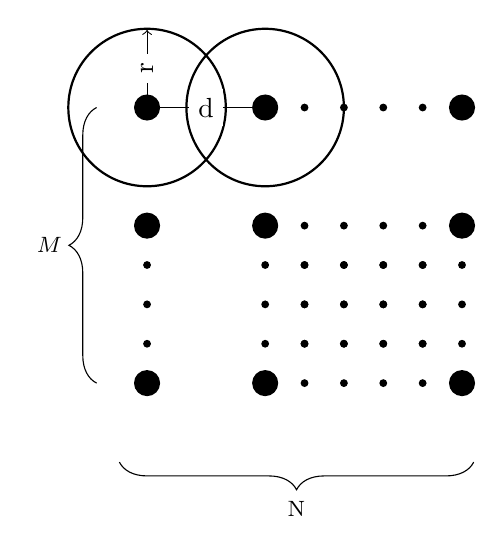
\begin{tikzpicture}
\draw(0,0) node[circle,fill=black]{};
\draw(1.5,0) node[circle,fill=black]{};

\draw(0,2) node[circle,fill=black]{};
\draw(1.5,2) node[circle,fill=black]{};
\draw(0,3.5) node[circle,fill=black]{};
\draw(1.5,3.5) node[circle,fill=black]{};
\foreach \x in {0,1.5,2,2.5,3,3.5,4}
    \foreach \y in {0.5,1,1.5} 
  {
       \node [fill,circle,scale=0.3]  (\x\y) at (\x,\y) {};} 
\draw(4,0) node[circle,fill=black]{};
\draw(4,2) node[circle,fill=black]{};
\draw(4,3.5) node[circle,fill=black]{};
\foreach \x in {2,2.5,3,3.5}
    \foreach \y in {0,0.5,1,1.5,2,3.5} 
  {
       \node [fill,circle,scale=0.3]  (\x\y) at (\x,\y) {};} 
       
       \draw[thick](0,3.5) circle(1cm);
       \draw[|->|, rotate around with nodes={90:(0,3.5)}]
       (0,3.5)--(1,3.5) node[midway,fill=white,rotate with]{r};
       \draw[|<->|](0,3.5)--(1.5,3.5) node[midway,fill=white]{d};
       \draw[thick](1.5,3.5) circle(1cm);
       
\draw [decorate,decoration={brace,amplitude=10pt},xshift=-4pt,yshift=0pt]
(-0.5,0) -- (-0.5,3.5) node [black,midway,xshift=-0.6cm] 
{\footnotesize $M$};

\draw [decorate,decoration={brace,mirror,amplitude=10pt},xshift=-1em,yshift=-2em](0,-0.3) -- (4.5,-0.3) node [black,midway,yshift=-0.6cm]{\footnotesize N};


\end{tikzpicture}
\centering
\caption{A M $\times$ N grid having a sensor with field of view r and distance between the nodes being d.}
\label{fig:Grid}
\end{figure}



With the newly computed energy data stream, we compute the cross correlation between all the sensors using equation \ref{eq:corrcoeff}
\begin{equation}
\label{eq:corrcoeff}
r(x,y)=\frac{\sum_{i=1}^{n}(X_i-\overline{X})(Y_i-\overline{Y})}{\sqrt{\sum_{i=1}^{n}(X_i-\overline{X})^2}\sqrt{\sum_{i=1}^{n}(Y_i-\overline{Y})^2}} \\
\end{equation}
$X$ and $Y$ are data streams.\\
$\overline{X}$ and $\overline{Y}$ is the mean value of $X$ and $Y$ respectively.\\
$n$ is the number of samples.\\






\section{Grid Correlation Sum}
\label{sec:gcs}
Using the cross correlation values between the sensors, we define correlation matrix $R$ between the $n$ sensor nodes as shown in the equation \ref{eq:corrMatrix} .
\begin{equation}
\label{eq:corrMatrix}
\centering
R = 
\begin{bmatrix}
    r(1,1) & r(1,2) & \dots  & r(1,n) \\
    r(2,1) & r(2,2)  & \dots  & r(2,n) \\
    \vdots & \vdots  & \ddots & \vdots \\
    r(n,1) & r(n,2)  & \dots  & r(n,n)
\end{bmatrix}
\end{equation}\\
r($\alpha$,$\beta$) represents correlation value between the sensor $\alpha$ and $\beta$.\\

Using correlation matrix($R$) and grid adjacency matrix(GAM) we define a quantity called \textit{Grid Correlation Sum (GCS)} as given in the equation \ref{eq:gridCorrelationSum}. GCS represents the sum of correlation value of the sensor pair residing on neighboring vertices of the grid.
As the matrices are symmetrical along the diagonals we only consider the elements of the upper triangle of the matrices excluding the diagonal elements. 

\begin{equation}
\centering
\text{GCS}=\sum_{i=1}^{n-1}\sum_{j=i+1}^{n}\text{R}(\phi(i),\phi(j))  \times \text{ GAM(i,j)}
\label{eq:gridCorrelationSum}
\end{equation}
$i,j$ represent $ i^{th}$ and $ j^{th}$ vertex on the grid.\\
$\phi$ is a mapping functions which gives the sensor present at vertex i.\\
$R(\alpha,\beta)$: correlation coefficient between the sensor $\alpha$ and $\beta$.\\
GAM:  Adjacency matrix of the grid as per definition \ref{def:GAM}.\\

We use GCS to identify the correct arrangement out of all the $N$ possible arrangement. If we compute  GCS for all the possible arrangements, the arrangement with the maximum GCS will represent the actual arrangement of the sensors on the grid.  
If two non neighboring sensors are kept on neighboring verticies or vice versa then the correlation value between those two sensors will be low and thus decreasing the GCS.
To illustrate this consider a sensor grid as shown in the figure \ref{fig:arrangement1}.
 It consists of 3 $\times$ 3 grid.  
GCS for the  the grid is :\\
\begin{equation*}
GCS_{1}=\text{r(1,2)+ r(1,4)+...r(2,3)+...r(5,6)+r(6,9)..+r(8,9)}
\end{equation*}

Now consider the arrangement shown in figure \ref{fig:arrangement2}, where the position of the sensors 3 and 6 are interchanged\\
\begin{equation*}
GCS_{2}=\text{ r(1,2)+r(1,4)+...+\textbf{r(2,6)}+...+\textbf{r(3,5)+r(3,9)}...+r(8,9)}
\end{equation*}

\begin{figure}[!ht]
\begin{floatrow}
\ffigbox{
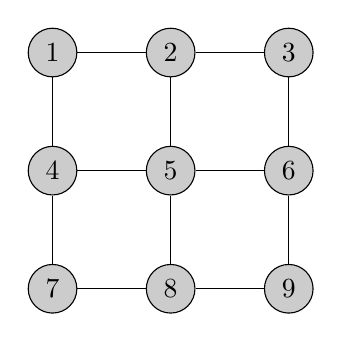
\begin{tikzpicture}[darkstyle/.style={circle,draw,fill=gray!40,minimum size=5}]
\foreach \y in {0,1,2}
 \foreach \x in {0,1,2}
{\pgfmathtruncatemacro{\label}{\x-3*\y+7}
\node[darkstyle](\x\y) at (1.5*\x,1.5*\y){\label};
}
 \foreach \x in {0,1,2}
    \foreach \y [count=\yi] in {0,1}  
      \draw (\x\y)--(\x\yi) (\y\x)--(\yi\x) ;

\end{tikzpicture}

\caption{Correct arrangement}
\label{fig:arrangement1}
}

\ffigbox{
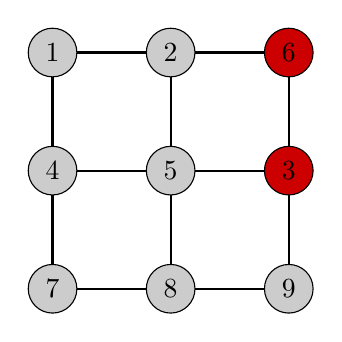
\begin{tikzpicture}[darkstyle/.style={circle,draw,fill=gray!40,minimum size=5}]

\draw[step = 1.5,thick ] (7.4,0) grid (10.5,3);
\node[circle,draw=black,fill=white!80!black,minimum size=5] (7) at (7.5,0) {7};
\node[circle,draw=black,fill=white!80!black,minimum size=5] (4) at (7.5,1.5) {4};
\node[circle,draw=black,fill=white!80!black,minimum size=5] (1) at (7.5,3) {1};

\node[circle,draw=black,fill=white!80!black,minimum size=5] (8) at (9,0) {8};
\node[circle,draw=black,fill=white!80!black,minimum size=5] (5) at (9,1.5) {5};
\node[circle,draw=black,fill=white!80!black,minimum size=5] (2) at (9,3) {2};

\node[circle,draw=black,fill=white!80!black,minimum size=5] (9) at (10.5,0) {9};
\node[circle,draw=black,fill=red!80!black,minimum size=5] (3) at (10.5,1.5) {3};
\node[circle,draw=black,fill=red!80!black,minimum size=5] (6) at (10.5,3) {6};
%\draw [<->,red] (3.east) to [out=60,in=60] (6.east);

\end{tikzpicture}

\caption{Incorrect arrangement}
\label{fig:arrangement2}
}
\centering

\end{floatrow}
\end{figure}

$GCS_{1}$ will be greater than $GCS_{2}$ as r(2,3) $>$ r(2,6) ,r(5,6)$>$r(3,5) and r(6,9) $>$ r(3,9) as sensors 2 and 6 , 3 and 5, 3 and 9 are non neighboring sensor nodes placed on neighboring vertices. Hence we can say that GCS will be maximum for a  mapping which maps sensors onto the grid accurately.\\
When the number of sensors is low we can identify the correct mapping by computing the GCS value for all the possible $N$ mappings. As the number of sensors increase the possible mappings to be checked also increases. Hence we need to find a method to reduce the search space.

\section{Maximum spanning Tree}

Having established a criterion to determine the right arrangement of sensors on the grid from  possible ${N}$ arrangements. The next step is to reduce the search space. For which we compute the maximum spanning tree (MST) for the correlation matrix ${R}$. 
If we consider ${R}$ as an adjacency matrix for a graph ${G}$, then the sensors represents the vertices and the correlation values between the sensors represents the weights of the edges between the corresponding sensors.
Now if we compute a maximum spanning tree for the graph, then the tree consists of all the sensor nodes connected to atleast one other node by an edge. The MST chooses an edge for every sensor such that the weight of the edge outgoing from the sensor $\alpha$ to sensor $\beta$ is the maximum among all the edges starting from sensor $\alpha$, in graph ${G}$. As the weights represent correlation values it implies that the maximum spanning tree connects a node to another with which it has the maximum correlation. As the correlation between the neighboring nodes is maximum we can say that MST connects the neighboring sensors.\\
 To compute the MST we make use of Prim's algorithm\cite{BLTJ:BLTJ1515}. As Prim's algorithm was originally developed to compute the minimum spanning tree we negate the weights for the correlation matrix and obtain the minimum spanning tree which will represent the maximum spanning tree for the original graph ${G}$. \\
As the sensors are placed on the grid and there exists an edge between the neighboring vertices of the grid. The MST over ${R}$ represents one of the spanning tree for the grid. As illustrated in the figure \ref{fig:MST}.
It is possible that for a given grid there may be several spanning trees with the same structure. 
Figure \ref{fig:variousMappings} shows few of the spanning tree similar to the MST obtained for the correlation matrix.
If we compute all the possible spanning trees for the grid which maintains the same structure as that of the maximum spanning tree for the correlation matrix and map each vertex on the MST to the corresponding spanning tree of the grid as shown in the figure \ref{fig:mapping}, we obtain several possible mappings of the sensors to grid location.Among the possible mappings we have to choose the correct arrangement. To choose the true arrangement of the sensor on the grid we make use of  GCS. The number of arrangements that are obtained from this method is lesser than the ${N}$  possible arrangements that we had to check previously. \\
The main reason for decrease in the possible mapping can be explained as follows:
When we are computing various mappings between the sensors maximum spanning tree and spanning tree for the grid suppose we assign one of the nodes($S_x$) on the  spanning tree to one of the nodes on the grid($G_x$) then in the next step the node which is connected to $S_x$ can be mapped only to the neighboring nodes of the grid node $G_x$ .









%Having established a method to determine the true arrangement of the sensor nodes on the grid from all the possible \textbf{N} arrangements, the next step is to prune the possible arrangements. \\
%From the definitions of neighboring sensors and neighboring vertices we can say that two neighboring sensors will always be placed on the neighboring vertices. From the grid adjacency matrix we can determine the neighboring vertices of a vertex. If we can determine the neighboring sensor nodes then we can prune the number of possible arrangements by using the constraints that only neighboring sensors can occupy the neighboring vertices. 




%If the neighbors of a sensor are known , the sensors occupying the neighboring vertices on the grid has to be occupied by it's neighboring sensors .
%The neighboring vertices of a vertex \textbf{i} on which a sensor \textbf{a} is located should be occupied by the neighbors of sensor \textbf{a}.
%Thus resulting in the reduction of the number of possible arrangements.

%If we know which are all the neighbors of a sensor then when a sensor is placed on the vertex of a sensor, we know that the neighboring vertex on the grid should only be occupied by it's neighboring nodes. 

%Though the correlation value between two neighboring nodes are high compared to the correlation value between the non neighboring nodes, finding a threshold to differentiate between the neighboring and non neighboring nodes when the arrangement is not known is non trivial.\\
%Although we might not be able to identify all the neighboring nodes even if we are able to find a minimum of one neighboring node per node we will be able to reduce the number of mappings that needs to be checked. To achieve this we calculate the maximum spanning tree for the correlation matrix \textbf{R}.

%If we consider R as an adjacency matrix with each sensor representing a vertex and the correlation value between the sensors representing the edge weight between them. Then the maximum spanning tree for such a graph will connect all the vertices together such that the total weight for the edges in the tree is maximum. 


%A maximum spanning tree has an edge between 2 nodes which have high correlation matrix compared with the other nodes. Therefore if an edge exists between two nodes in the maximum spanning tree then we can say that those two nodes are neighboring nodes.\\
%To compute the maximum spanning tree we use Prim's algorithm \cite{BLTJ:BLTJ1515}.Originally  Prim's algorithm is designed to compute the minimum spanning tree for a graph. In order to compute the maximum spanning tree the correlation matrix is negated and given as the input to the algorithm. The minimum spanning tree %obtained from negated weights is the maximum spanning tree for the original weights.This maximum spanning tree represents one of the spanning tree for the grid as can be seen from the figure \ref{fig:MST}. 

%A Maximum spanning tree chooses an edge which has the maximum weight starting from the vertex, among all the vertices that are present. As in our case the vertices represent the sensor nodes and edge weights is the correlation value between the sensor nodes. So  edge that is originates from the node connects to a node which is it's neighbor . As this step is carried on for every sensor , we have an edge originating from the sensor node, lets call it  the start node ending a sensor node, lets call it end node. The start node has the highest correlation with the end node. As the correlation values who are neighbors are the highest, we can safely tell %that this edge is connecting the start node to a neighbor of the start node.

%While computing the maximum spanning tree an edge from a node under consideration is chosen which has the maximum weight originating from it. out of all the edges the node has, the edge with the maximum weight is chosen. 

%While computing a maximum spanning tree an edge from a node is chosen which has the maximum weight compared to the other edges of the node under consideration. This process is repeated for all the nodes that are present in the graph. In our case each vertex represents a sensor and the edge weight is given by the cross %correlation value between the two sensors. Since for every node a maximum correlation value is chosen and as the correlation value between the neighbors is maximum we can say that in a maximum spanning tree two  neighboring sensors are connected. 

\begin{figure}[!ht]
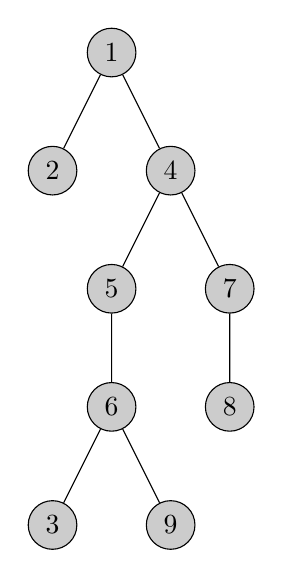
\begin{tikzpicture}[darkstyle/.style={circle,draw,fill=gray!40,minimum size=5}]
\node[darkstyle]{1}
	child{node[darkstyle]{2}}
    child{node[darkstyle]{4}
    	child{node[darkstyle]{5}
	        child{node[darkstyle]{6}
            	child{node[darkstyle]{3}}
                child{node[darkstyle]{9}}}}
                child{node[darkstyle]{7}
                child{node[darkstyle]{8}}}};
\end{tikzpicture}
\qquad \qquad \qquad
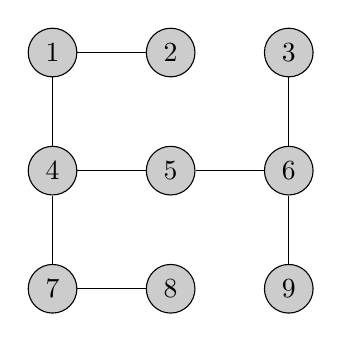
\begin{tikzpicture}[darkstyle/.style={circle,draw,fill=gray!40,minimum size=5}]
\foreach \y in {0,1,2}
 \foreach \x in {0,1,2}
{\pgfmathtruncatemacro{\label}{\x-3*\y+7}
\node[darkstyle](\x\y) at (1.5*\x,1.5*\y){\label};
}
\draw (01)--(02) (02)--(12) (01)--(11) (11)--(21) (21)--(22)
(21)--(20) (00)--(01) (00)--(10);


\end{tikzpicture}
\caption{A maximum spanning tree incident on the grid}
\label{fig:MST}
\end{figure}

\begin{figure}[!ht]

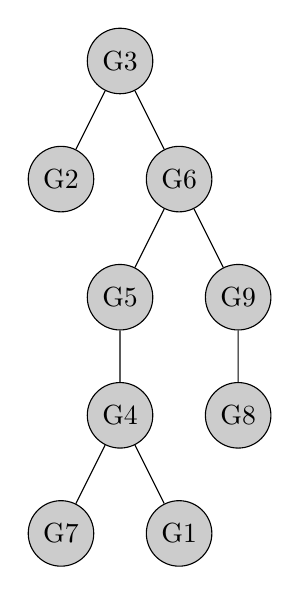
\begin{tikzpicture}[darkstyle/.style={circle,draw,fill=gray!40,minimum size=5}]
\node[darkstyle]{G3}
	child{node[darkstyle]{G2}}
    child{node[darkstyle]{G6}
    	child{node[darkstyle]{G5}
	        child{node[darkstyle]{G4}
            	child{node[darkstyle]{G7}}
                child{node[darkstyle]{G1}}}}
                child{node[darkstyle]{G9}
                child{node[darkstyle]{G8}}}};
\end{tikzpicture}
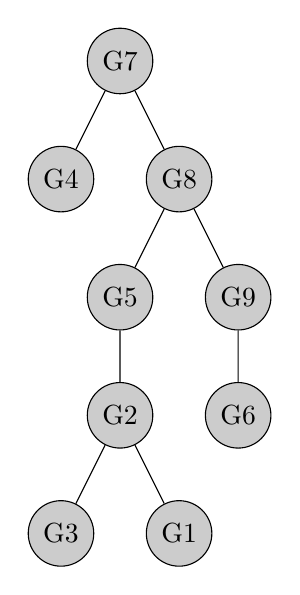
\begin{tikzpicture}[darkstyle/.style={circle,draw,fill=gray!40,minimum size=5}]
\node[darkstyle]{G7}
	child{node[darkstyle]{G4}}
    child{node[darkstyle]{G8}
    	child{node[darkstyle]{G5}
	        child{node[darkstyle]{G2}
            	child{node[darkstyle]{G3}}
                child{node[darkstyle]{G1}}}}
                child{node[darkstyle]{G9}
                child{node[darkstyle]{G6}}}};
\end{tikzpicture}
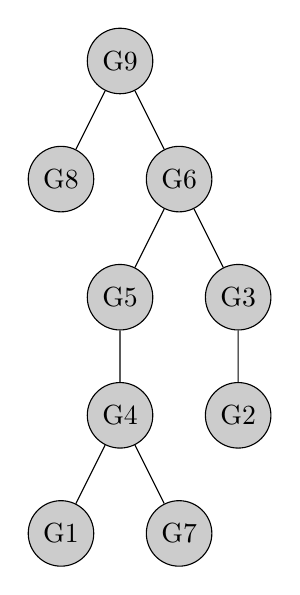
\begin{tikzpicture}[darkstyle/.style={circle,draw,fill=gray!40,minimum size=5}]
\node[darkstyle]{G9}
	child{node[darkstyle]{G8}}
    child{node[darkstyle]{G6}
    	child{node[darkstyle]{G5}
	        child{node[darkstyle]{G4}
            	child{node[darkstyle]{G1}}
                child{node[darkstyle]{G7}}}}
                child{node[darkstyle]{G3}
                child{node[darkstyle]{G2}}}};
\end{tikzpicture}
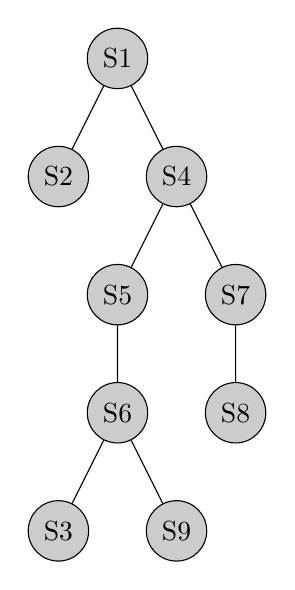
\begin{tikzpicture}[darkstyle/.style={circle,draw,fill=gray!40,minimum size=5}]
\node[darkstyle]{S1}
	child{node[darkstyle]{S2}}
    child{node[darkstyle]{S4}
    	child{node[darkstyle]{S5}
	        child{node[darkstyle]{S6}
            	child{node[darkstyle]{S3}}
                child{node[darkstyle]{S9}}}}
                child{node[darkstyle]{S7}
                child{node[darkstyle]{S8}}}};
\end{tikzpicture}
\caption{Various spanning tree for the grid with similar structure of the MST of the correlation matrix.}
\label{fig:variousMappings}
\end{figure}







\begin{figure}[!ht]
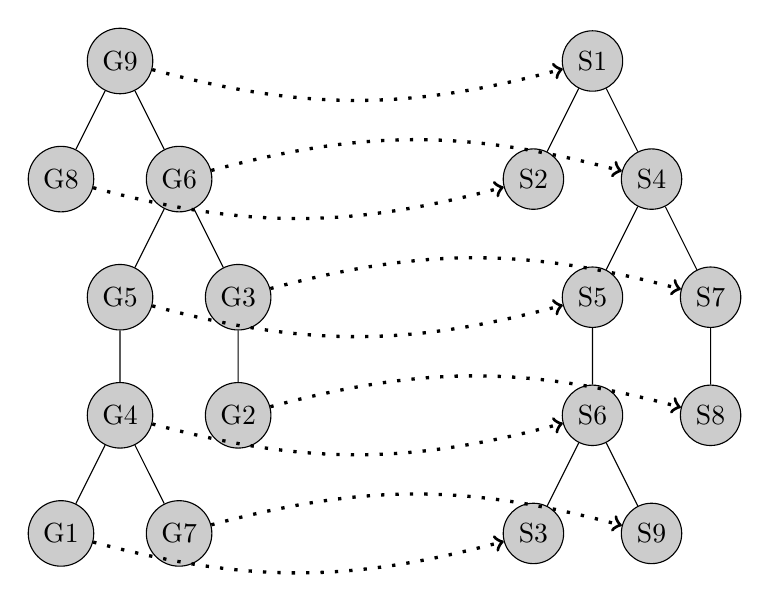
\begin{tikzpicture}[darkstyle/.style={circle,draw,fill=gray!40,minimum size=5}]
\begin{scope}
\node[darkstyle](G9){G9}
	child{node[darkstyle](G8){G8}}
    child{node[darkstyle](G6){G6}
    	child{node[darkstyle](G5){G5}
	        child{node[darkstyle](G4){G4}
            	child{node[darkstyle](G1){G1}}
                child{node[darkstyle](G7){G7}}}}
                child{node[darkstyle](G3){G3}
                child{node[darkstyle](G2){G2}}}};
\end{scope}
\qquad
\begin{scope}[shift={(6,0)}]
\node[darkstyle](S1){S1}
	child{node[darkstyle](S2){S2}}
    child{node[darkstyle](S4){S4}
    	child{node[darkstyle](S5){S5}
	        child{node[darkstyle](S6){S6}
            	child{node[darkstyle](S3){S3}}
                child{node[darkstyle](S9){S9}}}}
                child{node[darkstyle](S7){S7}
                child{node[darkstyle](S8){S8}}}};
\end{scope}
\draw[loosely dotted,very thick,->] (G9)to[out=0-15,in=195](S1);
\draw[loosely dotted,very thick,->] (G8)to[out=0-15,in=195](S2);
\draw[loosely dotted,very thick,->] (G6)to[out=15,in=165](S4);
\draw[loosely dotted,very thick,->] (G5)to[out=0-15,in=195](S5);
\draw[loosely dotted,very thick,->] (G4)to[out=0-15,in=195](S6);
\draw[loosely dotted,very thick,->] (G1)to[out=0-15,in=195](S3);
\draw[loosely dotted,very thick,->] (G7)to[out=15,in=165](S9);
\draw[loosely dotted,very thick,->] (G3)to[out=15,in=165](S7);
\draw[loosely dotted,very thick,->] (G2)to[out=15,in=165](S8);
\end{tikzpicture}
\caption{Mapping between the grid spanning tree and the MST for the correlation matrix}
\label{fig:mapping}
\end{figure}

% Graph monomorphism 

\section{Graph Matching} 

In the previous section we obtain a maximum spanning tree from the correlation matrix and saw how this represents a spanning tree for the grid. We also saw that there can multiple spanning tree whose structure is similar to the MST obtained for the correlation matrix. In this section we describe method to obtain all the possible spanning trees that has the same structure as the MST obtained from the correlation matrix of the sensors.
The task of checking if a pattern graph H is contained in a base graph G and obtaining all the mappings from G to H is a standard problem of graph matching.\\

A graph matching process between two graphs $G$ = $(V_G,E_G)$ and H = $(V_H,E_H)$ consists of determining a mapping M which associates nodes of the graph G to H and vice versa. Different constraints can be imposed onto M which results in different mapping types: monomorphism, isomorphism, graph-subgraph isomorphism are the most popular ones. Our problem falls under the category of graph monomorphism . \\
Two graphs 
 $G =( V_G, E_G)$ and
 H =$( V_H, E_H)$  are monomorphic  if and only if there exists an injective (node)
mapping $\phi (V_G) \rightarrow  V_H$ : for which $\forall v,w \in V_G:(v,w) \in E_G \Rightarrow (\phi((v),\space \phi(w)) \in E_H.$\\  

Monomorphism is often confused with subgraph isomorphism. Monomorphism is a weaker kind of subgraph isomorphism. \\
Two graphs  $G =( V_G, E_G)$ and
 H =$( V_H, E_H)$  are sub graph isomorphic  if and only if there exists an injective (node)
mapping $\phi( V_G) \rightarrow  V_H$ : for which $\forall \text{ v,w} \in V_G:(v,w) \in E_G \Leftrightarrow (\phi((v),\space \phi(w)) \in E_H.$ 
The relationship between edges of the graphs are equivalence for subgraph isomorphism, and for Monomorphism  relationship  is an implication.\\
A problem of finding all the Monomorphisms of the pattern graph into the base graph is defined as Monomorphism problem. Graph Monomorphism is a NP-Complete problem \cite{Garey:1979:CIG:578533}. 
\subsection{Related Work}

Graph matching is widely used in pattern recognition and image processing applications. Graph matching also finds its application in the field of biomedical and biological applications. 
Most of the algorithms for graph matching are based on some form of tree search with backtracking.
 The basic idea is that the partial mapping (initially empty) is iteratively expanded by adding to it new pairs of matched nodes; the pairs are chosen based on some conditions employed to satisfy the conditions of the matching type.

The key principle is that there will be a partial mapping(initially empty)and is expanded iteratively by adding to it a new pairs of matched node. The matched nodes are chosen based on the certain conditions that depend on the matching type.

The first prominent and one of the most widely used algorithm in the area of graph matching was proposed by \citeauthor{Ullmann:1976:ASI:321921.321925} \cite{Ullmann:1976:ASI:321921.321925}. Ullmann algorithm addresses the problem of graph isomorphism, sub graph isomorphism , graph monomorphism. Ullmann algorithm is based on  depth first search with backtracking. To prune unfruitful matches the author proposes a refinement procedure, which employ conditions based on the knowledge of the adjacent nodes and the degree of the nodes that are being matched. 
\citeauthor{4308468} in \cite{4308468} propose a graph monomorphism algorithm. The authors formulate the graph monomorphism problem as a minimum weight clique problem of weighted nets . The major drawback of the algorithm is that the algorithm uses a $N^2 \times N^2$ matrix to represent netgraph
. N representing the number of nodes of the largest graph. As a result of this only small graphs can be dealt with using the algorithm.  
A more recent algorithm for graph isomorphism, subgraph isomorphism and monomorphism was proposed by \citeauthor{906251} in \cite{906251}, popular as VF algorithm. The authors define a heuristic that is based on the analysis of sets of nodes adjacent to the ones already considered in the partial mapping. The authors further improved the algorithm in 2001 in their paper \cite{cordella2001improved}. 
The authors proposed a modification to the algorithm and called it VF2. The authors introduce a method to restore data structure, which enabled them to reduce the memory consumption from $O(N^2)$ to O(N) where N is the number of nodes in the graph, thus enabling the algorithm to work with large graphs.
In our work we use the VF2 algorithm to obtain the mappings between the spanning tree and grid graph.

\subsection{VF2}

In this section we give a brief description about VF2 algorithm.\\

\begin{figure}

\begin{algorithm}[H]
\begin{algorithmic}
 \LState  \textbf{Procedure} Match(s)\\
\textbf{INPUT:}  an intermediate state s; the initial state $s_0$ has $M(s_0)=\emptyset$\\
\textbf{OUTPUT:} the mappings between two graphs\\
\textbf{Match(s)}\\
 \textbf{IF} M(s) covers all the nodes of $G_2$ \textbf{THEN}\\
\quad \textbf{OUTPUT} M(s)\\
\textbf{ELSE}\\
 \quad    Compute the set P(s) of the pairs of candidates for inclusion in M(s)\\
\quad\textbf{FOREACH} (n,m) $\in$ P(s)\\
\quad\quad\textbf{IF} F(s,n,m) \textbf{THEN}\\
\quad\quad\quad	Compute the state s' obtained by adding (n,m) to M(s)\\
\quad\quad\quad\textbf{CALL} Match(s')\\
\quad\quad\textbf{ENDIF}\\
\quad\textbf{ENDFOREACH}\\
\quad Restore data structure\\
\textbf{ENDIF}\\

\end{algorithmic}
\end{algorithm}
\caption{Pseudo code for VF2 algorithm}
\label{fig:VF2}
\end{figure}


% VF2 explanation 
VF2 algorithm is a graph matching algorithm to solve graph isomorphism, monomorphism and  subgraph isomorphism problem. VF2 uses depth search first method to iterate through all the nodes and recursive backtracking technique to check for all the possible mappings. A process of matching 
a base graph G to a pattern graph H consists of determining a mapping M which associate nodes of base graph (G) with nodes of the pattern graph (H) and vice versa, with some constraints.
Mapping is expressed as a set of pairs of node (n,m) with n $\in$ G and m $\in$ H. 
In VF2 algorithm the process of finding the mapping function is described by a  State Space Representation (SSR). Each state s of the matching process can be associated to a partial mapping solution M(s),
which contains only a subset of M. A transition from current state(s) to the next state(s') represents the addition of a mapping (n,m) to the state s.

VF2 algorithm introduces a set of rules which helps to prune the number of possible SSR that needs to be checked before obtaining a valid mapping. Figure \ref{fig:VF2} gives a high-lvel description of the VF2 algorithm.
There are 3 important functionalities in the algorithm: 
\begin{itemize}
\item generation of possible mappings(P(s)) .
\item checking of the validity of the mapping(F(s,n,m)).
\item Restore data structure.
\end{itemize}


%Data graph (G), Querry graph(Q)

\subsection{Computation of candidate pair set P(s)}
This section explains the method to compute the candidate pair set P(S) for an undirected graph G and H. 
For every intermediate state s the algorithm computes P(s), a set of possible mapping pairs. For each pair p belonging to P(s) the feasibility of its addition F(s,n,m) is checked : if the check is successful the next state $s' = s \cup p$ and the whole process recursively applies to s'.

To compute P(S) set $T_1(s)$ and $T_2(s)$ are defined for Graph G and H respectively. $T_1$ and $T_2$ are the set of  nodes in G and H, which are neighbors of the set of nodes included in the partial mapping state M(s) but are not included in M(s).
Set P(s) will be made of all the the node pairs(n,m) with n being a node in $T_1$ with the smallest label  and m being a node in $T_2$ . If  $T_1$ and $T_2$ sets are empty then the set P(s) be calculated by using the sets of nodes not contained in either G(s), H(s).

\subsection{Feasibility Rules}
Feasibility Rules are used to check the consistency of the partial solution s' obtained by adding nodes n,m and prune the search tree. The functionality of the rules are as explained below.

In vf2 algorithm, those candidates(m,n) are pruned if m is not connected to already matched nodes in $G_q$
(i.e nodes of $G_q$ included in M(s)).
Subsequently, the pruning step also removes those node-pairs(m,n) in which n is not connected to the matched 
nodes in the data Graph G. These pruning rules assume that the query and data graph are connected.\\

The algorithm also compares the number of neighboring nodes of each n and m that are connected to nodes in M(s) but are not
included in M(s). The number of such nodes in the data graph must be greater than or equal to the number of such nodes in the query graph.\\

Finally the number of neighboring nodes of each of n and m that are not directly connected to nodes in M(s) are compared. The number of 
such nodes in the data graph must be greater than or equal to the number of such nodes in the query graph.

\subsection{Restore data structure}
In VF2 algorithm all the vectors that are used to store data have the following property: If an element is non-null in a state s, it will remain non-null in all states descending from s. This property, together with the depth-first strategy of the search is, is used to avoid the need to store a different copy of the vectors for each state: when the algorithm backtracks, it restores the previous value of the vectors. Hence the space complexity of VF2 algorithm is of the order O(N). This is illustrated in the figure \ref{fig:memManagement}.As can be seen at the last state if a variable was created at every state then we will end up with $N^2$ variables.

\begin{figure}
\includegraphics[scale=0.5]{./pics/memManagement.png}
\caption{Memory cells occupied at each state with and without restore data}
\label{fig:memManagement}
\centering
\end{figure}

\subsection{Computation Complexity}
Computational complexity of the VF2 depends on two factors: 
\begin{itemize}
\item The time required to calculate the feasibility of every SSR's , computation of the node pair mappings.
\item Number of SSR visited.
\end{itemize}

According to the authors the former has a time complexity of $O(N)$ . For the latter the authors consider a best case; where only only one of the potential mappings are feasible which makes the computation complexity $O(N)$ and thus making the overall complexity $O(N^2)$. In the worst case, the algorithm has to explore all the states. This can happen when every node is connected to every other node (base graph is a complete graph) and the graph exhibits strong symmetry. The authors show that the complexity in such a condition is $O(N!)$ and thus making the total complexity $O(N!N)$.
In our case we show the order of complexity for a 8-neighborhood grid. The worst case for such a grid will arise when at every stage of the search tree the algorithm has to explore every possible branch. Since it's a 8-neighborhood grid all the nodes except the ones at the edges of the grid will have 8 neighbors. As one of the neighboring node would be the parent node the node at stage $i$ will have $7^{i}$ possibilities to explore and stage N there will be $7^n$ possibilities to explore . The total number of states to explore will be given by the sum:\\

\begin{align*}
1 + 7 + 7^2+ . . . . .+7^i+....7^n\\
\text{This represents a geometric progression with a= 1, r =7.}\\
\text{Sum of a geometric progression is given by:}\\
S_{n}=\frac{a(r^n-1)}{r-1}\\
S_{n}=\frac{7^{n+1} -1}{7-1} \\
\text{When n is large}\\
S_{n} \approx 7^N\\
\end{align*}

Thus computational complexity is $O(7^NN)$

\begin{figure}
\includegraphics[scale=0.5]{./pics/tree.png}
\caption{All the visited states in case of a 8 neighborhood grid with n nodes.}
\label{fig:ccO}

\end{figure}

\section{Determination of sensor placement}
\label{ref:rotationalSym}
After we obtain the various mappings. We need to decide which out of the various mappings gives the actual placement of the sensors on the grid. To identify the correct mapping we compute GCS as explained in section \ref{sec:gcs}. We calculate the grid correlation sum for all the mappings obtained and the mappings which gives the maximum sum will be the actual placement of the sensors on the grid. 
\subsection{Limitations}

Our method  can identify the location of the sensors upto rotational symmetry. As the $GCS$ remains the same for a sensor arrangement which is rotationally symmetrically to the original sensor arrangements. 
As seen in the two arrangements that are shown in the figure \ref{fig:symm} and \ref{fig:rotationalSymm}. Therefore when we pick the mappings which has the highest GCS we get multiple mappings. These mappings include the actual arrangement and arrangement which are rotationally symmetric it.

\begin{figure}[!ht]
\begin{floatrow}
\ffigbox{
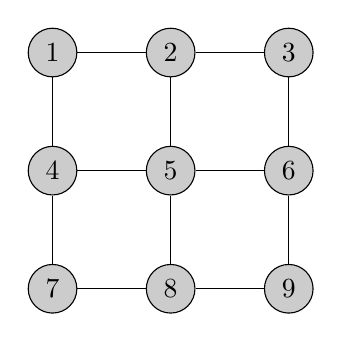
\begin{tikzpicture}[darkstyle/.style={circle,draw,fill=gray!40,minimum size=5}]
\foreach \y in {0,1,2}
 \foreach \x in {0,1,2}
{\pgfmathtruncatemacro{\label}{\x-3*\y+7}
\node[darkstyle](\x\y) at (1.5*\x,1.5*\y){\label};
}
 \foreach \x in {0,1,2}
    \foreach \y [count=\yi] in {0,1}  
      \draw (\x\y)--(\x\yi) (\y\x)--(\yi\x) ;

\end{tikzpicture}

\caption{Actual arrangement}
\label{fig:symm}
}


\ffigbox{
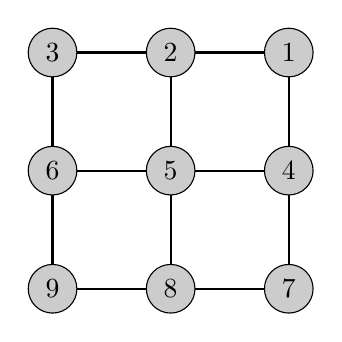
\begin{tikzpicture}[darkstyle/.style={circle,draw,fill=gray!40,minimum size=5}]

\draw[step = 1.5,thick ] (7.4,0) grid (10.5,3);
\node[circle,draw=black,fill=white!80!black,minimum size=5] (7) at (7.5,0) {9};
\node[circle,draw=black,fill=white!80!black,minimum size=5] (4) at (7.5,1.5) {6};
\node[circle,draw=black,fill=white!80!black,minimum size=5] (1) at (7.5,3) {3};

\node[circle,draw=black,fill=white!80!black,minimum size=5] (8) at (9,0) {8};
\node[circle,draw=black,fill=white!80!black,minimum size=5] (5) at (9,1.5) {5};
\node[circle,draw=black,fill=white!80!black,minimum size=5] (2) at (9,3) {2};

\node[circle,draw=black,fill=white!80!black,minimum size=5] (9) at (10.5,0) {7};
\node[circle,draw=black,fill=white!80!black,minimum size=5] (3) at (10.5,1.5) {4};
\node[circle,draw=black,fill=white!80!black,minimum size=5] (6) at (10.5,3) {1};
%\draw [<->,red] (3.east) to [out=60,in=60] (6.east);

\end{tikzpicture}

\caption{Sensors arrangement rotationally symmetric to the actual arrangement }
\label{fig:rotationalSymm}
}
\centering

\end{floatrow}
\end{figure}


\subsection{Special case when the grid is $n \times 2$ or $2 \times n$}
Consider a sensor $2 \times n$ sensor grid with diagonally opposite nodes connected as shown in the figure \ref{fig:ntime2}. These grid structure posses a special case of symmetry. As shown in the  figure \ref{fig:ntime2Sym} the nodes 1 and 2 are interchanged; it is as if the whole structure was rotated with  edge (1,2) fixed. The diagonally opposite edges (1,3) in figure \ref{fig:ntime2} becomes non diagonal edges in the figure \ref{fig:ntime2Sym}. To overcome this error we use weighted grid adjacency matrix instead of a binary grid adjacency matrix. We compute \textit{Weighted Grid Adjacecny Matrix (WGMA)} as follows:
First we normalize the distance between all the sensor nodes which has an edge between them in the $GAM$ by dividing all the distances between the sensor nodes by the minimum distance$(d_{min})$ that exists between the nodes in the entire grid. Then we take the reciprocal of the normalized distance to obtain the WGAM. All the members of the WGAM value lies between the 0 and 1. 1 signifying the 2 sensors are close to each other and 0 signifying that the 2 sensors are far away from each other.\\
\[
WGAM_{i,j} = 
\begin{cases}
\dfrac{d_{min}}{d_{i,j}}, &\text{ if } GAM_{i,j} = 1\\
0, & \text{otherwise}\\
\end{cases}
\]


We use $WGAM$ instead of $GAM$ to compute $GCS$ in equation \ref{eq:gridCorrelationSum}. The reasoning behind the use of WGAM matrix instead of the GAM is that we hypothesize that the correlation values for the sensor which are closer is higher than the one compared to sensors which are further apart. By assigning weights to the edges in this manner, more importance is given to the edges between the sensors that are closer to the each other. Doing so the sensors which are close by contribute  more to the $GCS$ . 
Now if we consider arrangement as shown in the figure \ref{fig:ntime2} and \ref{fig:ntime2Sym} though there $GCS$ remain the same with $GAM$, $GCS$ won't remain the same when $WGAM$ is used. The contribution of the correlation between the sensors placed on the non diagonal edges are more compared to the contribution made by the diagonal edges. Therefore if we place the non diagonally located sensors on the diagonals of the grid $GCS$ decreases. Thus by using a weighted grid adjacency matrix we are able to obtain the mapping of the sensors onto the grid upto rotational symmetry.

\begin{figure}
\begin{floatrow}
\ffigbox{

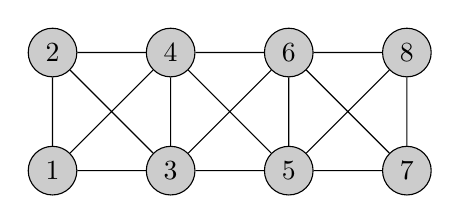
\begin{tikzpicture}

\node[circle,draw=black,fill=white!80!black,minimum size=5] (1) at (0,0) {1};
\node[circle,draw=black,fill=white!80!black,minimum size=5] (3) at (1.5,0) {3};
\node[circle,draw=black,fill=white!80!black,minimum size=5] (5) at (3,0) {5};
\node[circle,draw=black,fill=white!80!black,minimum size=5] (7) at (4.5,0) {7};
\node[circle,draw=black,fill=white!80!black,minimum size=5] (2) at (0,1.5) {2};
\node[circle,draw=black,fill=white!80!black,minimum size=5] (4) at (1.5,1.5) {4};
\node[circle,draw=black,fill=white!80!black,minimum size=5] (6) at (3,1.5) {6};
\node[circle,draw=black,fill=white!80!black,minimum size=5] (8) at (4.5,1.5) {8};
\draw (1)--(2) (1)--(3) (1)--(4) (2)--(3) (3)--(4) (4)--(6)   (2)--(4)  (4)--(5) (3)--(6) (3)--(5) (5)--(6) (6)--(7) (5)--(8) (5)--(7) (7)--(8) (8)--(6);
\end{tikzpicture}
\caption{Actual arrangement of $2 \times 4$ grid.}
\label{fig:ntime2}
}

\ffigbox{
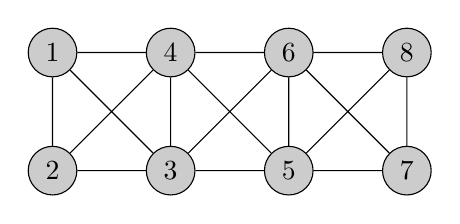
\begin{tikzpicture}
\node[circle,draw=black,fill=white!80!black,minimum size=5] (2) at (0,0) {2};
\node[circle,draw=black,fill=white!80!black,minimum size=5] (3) at (1.5,0) {3};
\node[circle,draw=black,fill=white!80!black,minimum size=5] (5) at (3,0) {5};
\node[circle,draw=black,fill=white!80!black,minimum size=5] (7) at (4.5,0) {7};
\node[circle,draw=black,fill=white!80!black,minimum size=5] (1) at (0,1.5) {1};
\node[circle,draw=black,fill=white!80!black,minimum size=5] (4) at (1.5,1.5) {4};
\node[circle,draw=black,fill=white!80!black,minimum size=5] (6) at (3,1.5) {6};
\node[circle,draw=black,fill=white!80!black,minimum size=5] (8) at (4.5,1.5) {8};
\draw (1)--(2) (1)--(3) (1)--(4) (2)--(3) (3)--(4) (4)--(6)   (2)--(4)  (4)--(5) (3)--(6) (3)--(5) (5)--(6) (6)--(7) (5)--(8) (5)--(7) (7)--(8) (8)--(6);


\end{tikzpicture}
\caption{Incorrect arrangement of $2 \times 4$ grid with the same $GCS$ values.}
\label{fig:ntime2Sym}
}
\centering
\end{floatrow}
\end{figure}


\section{Summary}
In this chapter we describe a method to locate the sensor on the grid making use of sensor data and grid vertices information up-to rotational symmetry. Figure \ref{fig:Summary} gives the summary of steps involved in the form of a flowchart. 

\begin{figure}
\includegraphics[scale=0.6]{./pics/methodSummary.png}
\caption{Flowchart for the method developed}
\label{fig:Summary}
\centering
\end{figure}



 






 



\chapter{Test Bed}
\label{chp:testbed}

We setup our testbed in a $8m\times6m$ office space. Sensors are mounted on the ceiling which is at a height of 3m. The sensors are  placed 2.5m apart in the horizontal direction and 2.2m apart in the vertical direction. We use  PIR sensor, EKMB1101112 from Panasonic. 
The output of the sensor is binary, with 1 indicating occupancy and 0 if the region is unoccupied.  We use the sensors with eZ430-RF2500 toolkit which consists of MSP430 micro-controller  and CC2500 multi-channel
RF transceiver for wireless communication. The testbed uses simpliciTI a TI proprietary  low-power RF network protocol. To avoid collision CSMA/CA is employed. We mount the 8 sensors on the ceiling of the room as shown in the figure \ref{fig:photo} with the sensors highlighted in red. A schematic representation of the lab is as shown in the figure \ref{fig:roomLayout}. All the 8 nodes communicate directly to a centrally located access point which is connected to a laptop, which stores the data.
To decrease the packet loss we enable acknowledgment. An acknowledgment (ack) is sent from the AP if the packets are received. If no ack is received by a node, the node retransmits its data a maximum of 6 times until an ack is  received from the AP. If no ack is received even after retransmission the packet is dropped and the node continues carrying on its function. From the figure \ref{fig:packetLoss} and table we can see that the there was a decrease in the packet loss per node after ack was enabled. 
\begin{figure}[!ht]
\includegraphics[scale=0.5]{./pics/lab_photo.jpg}
\caption{Photo of the lab setup with the sensors highlighted in red}
\label{fig:photo}
\end{figure}
\begin{figure}[!ht]
\centering
\includegraphics[scale=0.5]{./pics/roomLayout.png}
\caption{Room layout of the testbed.}
\label{fig:roomLayout}
\end{figure}

PIR sensors are sampled every 100ms. All the nodes have a local clock running on them. With 1 clock tick corresponding to 1ms. All the local clocks are synchronized to one global clock. Since the data is binary we combine 32 samples and transmit the packet every 3.2s. 
Data packet is an array of 8 bit. The packet structure is as shown in the figure \ref{fig:packetStructure}\\


\begin{figure}[!ht]
    \centering
    \begin{subfigure}[b]{1\textwidth}
        \centering
        \includegraphics[width=8cm,height=4cm]{./pics/packetLoss.png}
      \caption{Data before ack was enabled}
       % \label{fig:y equals x}
    \end{subfigure}
    \hfill
    \begin{subfigure}[b]{1\textwidth}
        \centering
        \includegraphics[width=8.5cm,height=4cm]{./pics/dataAfterAck.png}
        \caption{Data after ack was enabled}
        %\label{fig:three sin x}
    \end{subfigure}
\caption{Data from the test bed. - 1 indicates the lost data , 1 indicates occupancy, 0 indicates unoccupied space}
\label{fig:packetLoss}
\end{figure}

\begin{table}[!ht]
\centering
\caption{Packet loss without and with ack for all the sensor nodes}
\label{tab:packetLoss}
\begin{tabular}{|c|c|c|}
\hline
Node & \begin{tabular}[c]{@{}c@{}}Packet loss Without \\ ack(\%)\end{tabular} & Packet loss With ack(\%) \\ \hline
1    & 7.66                                                               & 0                    \\ \hline
2    & 1.01                                                             & 0                    \\ \hline
3    & 5.65                                                             & 0.32                 \\ \hline
4    & 23.67                                                            & 0                    \\ \hline
5    & 14.05                                                            & 0                    \\ \hline
6    & 1.48                                                             & 0                    \\ \hline
7    & 0.96                                                              & 2.20                    \\ \hline
8    & 4.54                                                             & 0                    \\ \hline
\end{tabular}
\end{table}

\begin{figure}[!ht]
 \bytefieldsetup{bitheight=3em}
\begin{bytefield}[bitwidth=2.5em]{14}
\bitheader{0-13} \\
\bitbox{1}{\tiny Mac id} & \bitbox{1}{\tiny packet number} &
\bitbox{4}{start time}
& \bitbox{4}{end time} & \bitbox{4}{data}
\end{bytefield}.
\caption{Packet Structure}
\label{fig:packetStructure}
\end{figure}
The transmitted packet is an array of 1 byte. Consisting of 14 bytes of payload. The payload structure is as shown in the figure \ref{fig:packetStructure}
\begin{itemize}
\item Mac Id - unique identifier for each node.
\item Packet number- Keeps track of the packets that are being transmitted from a  node. It helps to identify the lost packets as well as repeated packets.
\item Start time - 4 byte array corresponding to the time of first PIR sample of the PIR sensor in the packet.
\item End time - 4 byte array corresponding to the time of  last sample of the PIR sensor in the packet.
\item Data - 32 samples of the PIR sensor.
\end{itemize}

Data was collected for a span of 2 months. During the course of the evaluation, the occupants were notified of data gathering, but were never instructed to behave in any particular way or was there any constrained applied on the activity or the number of people in the room. 


\chapter{Results and Discussion}
In order to verify the proposed method we test our method with two datasets. First we apply our method to the data collected from the test bed which is described in the chapter \ref{chp:testbed} . Next we make use of the data released by the WSU smart home project\footnote{http://ailab.wsu.edu/casas/datasets/} \cite{cook2009assessing}.
\section{HTC34 testbed}
As described earlier the testbed consists of a 8 sensors arranged in a $4 \times 2$ grid. The sensor has a filed of view of radius 2.6m the calculation is explained in appendix \ref{app:fov}. The overlap between the field of view of sensors placed on the grid is as shown in the figure \ref{fig:fov} With the help of the co-ordinates of the sensors we obtain the adjacency matrix of the grid as shown in the figure \ref{fig:gamGraph}.
%\subsection{Determination of Window length}
%The first step in evaluation of our method is to obtain the energy stream from the raw data. To obtain the energy stream we use a moving window with 50\% overlap. We determine this window length empirically. As we already know the neighbors of every sensor
%We determine the window length empirically. We calculate 



\begin{figure}
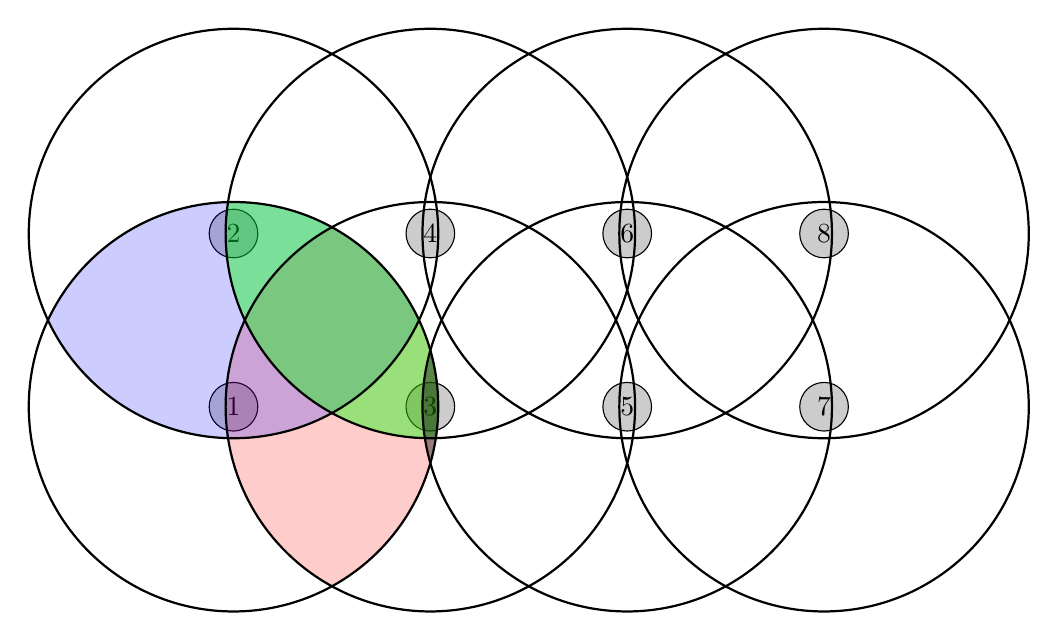
\begin{tikzpicture}
\node[circle,draw=black,fill=white!80!black,minimum size=5] (1) at (0,0)     {1} ;
\node[circle,draw=black,fill=white!80!black,minimum size=5] (3) at (2.5,0)   {3};
\node[circle,draw=black,fill=white!80!black,minimum size=5] (5) at (5,0)     {5};
\node[circle,draw=black,fill=white!80!black,minimum size=5] (7) at (7.5,0)   {7};
\node[circle,draw=black,fill=white!80!black,minimum size=5] (2) at (0,2.2)   {2};
\node[circle,draw=black,fill=white!80!black,minimum size=5] (4) at (2.5,2.2) {4};
\node[circle,draw=black,fill=white!80!black,minimum size=5] (6) at (5,2.2)   {6};
\node[circle,draw=black,fill=white!80!black,minimum size=5] (8) at (7.5,2.2) {8};

\begin{scope}
  \clip (0,0)      circle(2.6);
  \fill[red,fill opacity=.2] (2.5,0)    circle(2.6);
\end{scope}
\begin{scope}
  \clip (0,0)      circle(2.6);
  \fill[blue,fill opacity=.2] (0,2.2)    circle(2.6);
\end{scope}
\begin{scope}
  \clip (0,0)      circle(2.6);
  \fill[green,fill opacity=.4] (2.5,2.2)    circle(2.6);
\end{scope}
\begin{scope}
  \clip (0,0)      circle(2.6);
  \fill[black,fill opacity=.4] (5,0)    circle(2.6);
\end{scope}

\draw[thick](0,0)      circle(2.6);
\draw[thick](2.5,0)    circle(2.6);
\draw[thick](5,0)      circle(2.6);
\draw[thick](7.5,0)    circle(2.6);
\draw[thick](0,2.2)    circle(2.6);
\draw[thick](2.5,2.2)  circle(2.6);
\draw[thick](5,2.2)    circle(2.6);
\draw[thick](7.5,2.2)  circle(2.6);

\end{tikzpicture}
\centering
\caption{Overlapping field of view of the sensors on the vertex with the overlapping field of view for sensor 1 highlighted in color}
\label{fig:fov}
\end{figure}



\begin{figure}
\includegraphics[scale=0.5]{./pics/adjacency.png}
\caption{Grid adjacency matrix for the grid and its corresponding adjacency graph}
\label{fig:gamGraph}


\end{figure}

%\section{Convergence Time}
%An important aspect to know in an data driven method is to know how much of data is required in order to get accurate results. For this purpose we 
\section{Results}
The Grid adjacency matrix for the grid and corresponding grid graph is as shown in figure \ref{fig:gamGraph}. The computed correlation values for one of the dataset  is as shown in the figure \ref{fig:corrMatrix}.
We evaluate the performance with 10 different datasets. We were able to map the sensors onto the grid accurately upto rotational symmetry using the weighted grid adjacency matrix and calculating the $GCS$. The mappings obtained are as shown in the figure \ref{fig:arrangement}.
Table \ref{tab:resHTC} provides details about the number of states visited, number of mappings between the MST and the grid, and the number of mappings obtained as the solution from the developed method and the percentage error. As can be seen from table we obtain 0\% error for all the datasets. 
The number of states visited(includes all the intermediate states) and the number of mappings is lesser than number of possible arrangements which is $8! = 40320$. Number of mappings is almost 14 times lesser than brute force method.

\begin{figure}
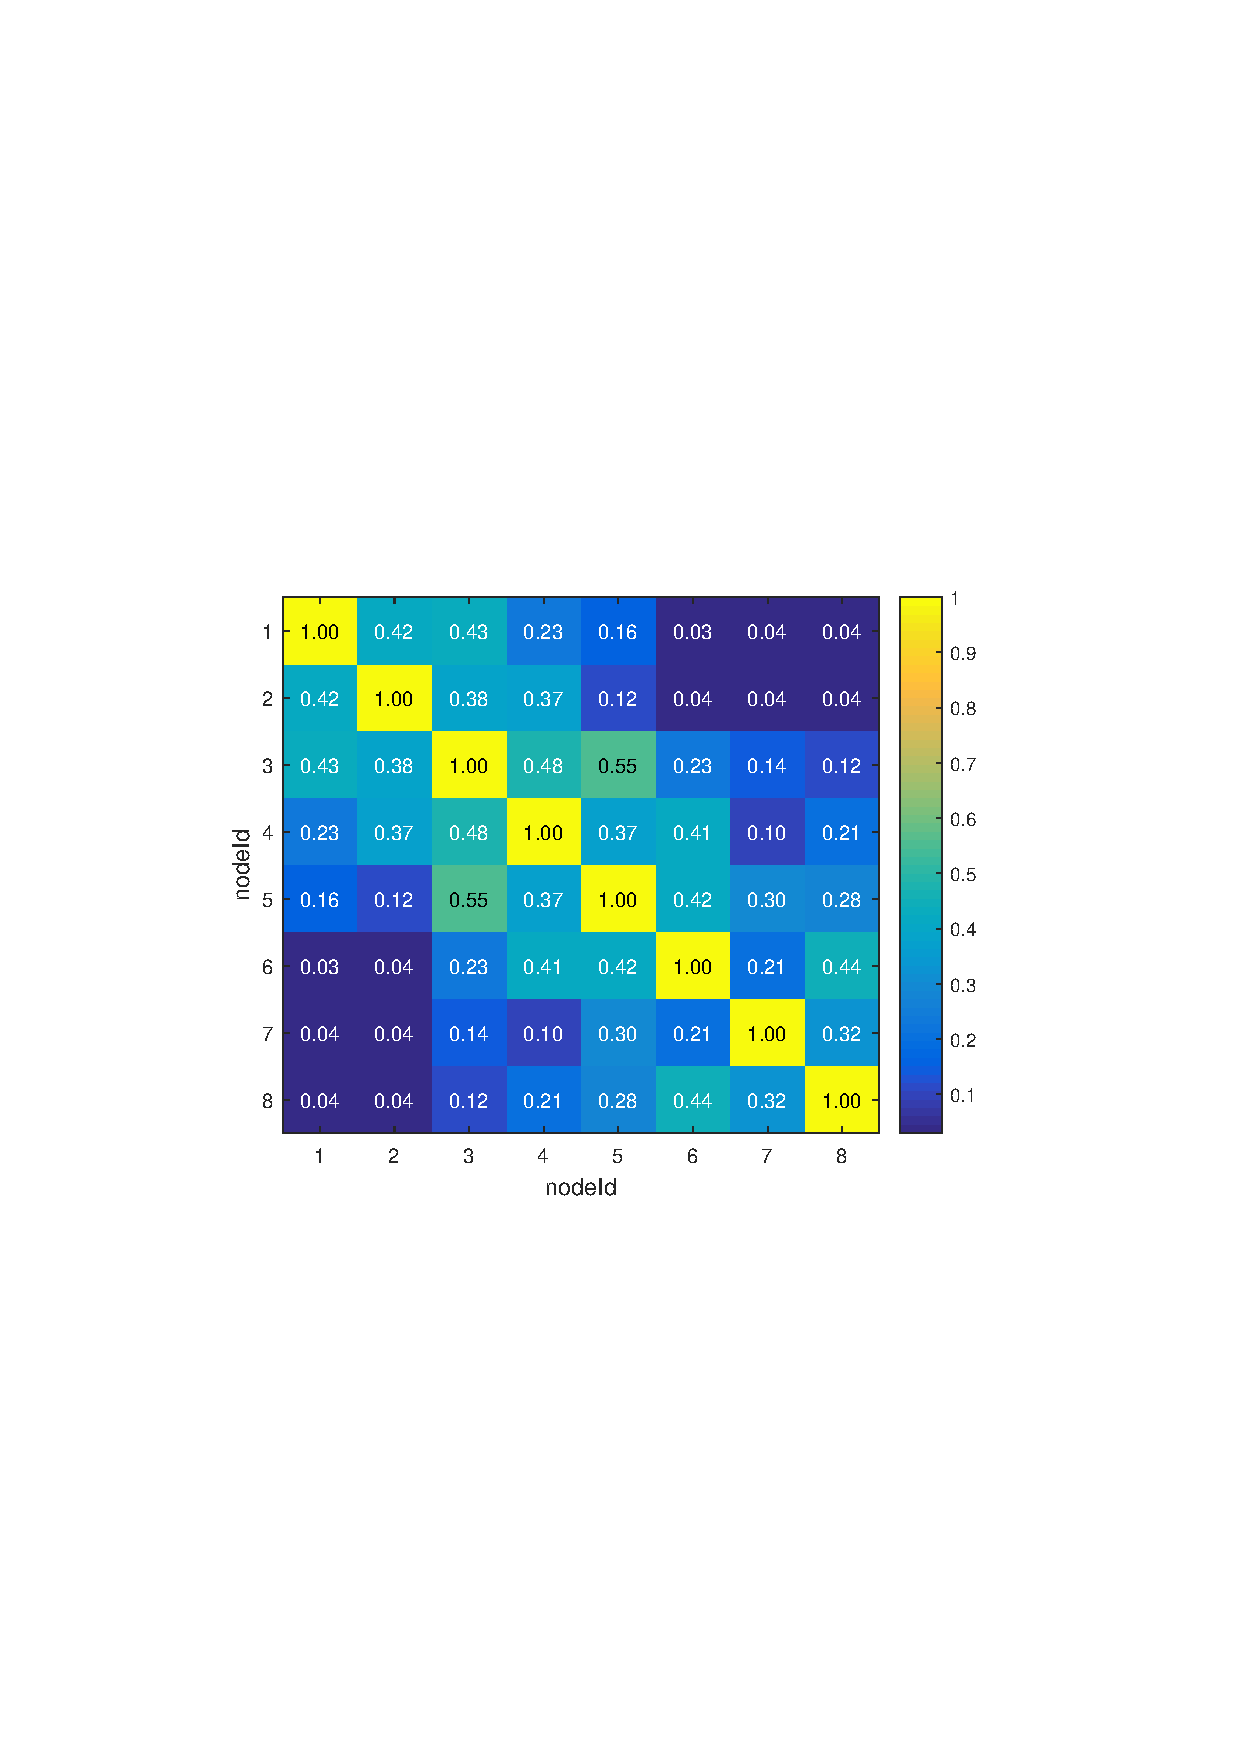
\includegraphics[scale=0.75]{./pics/correlation.pdf}
\caption{Correlation matrix R}
\centering
\label{fig:corrMatrix}

\end{figure}

\begin{table}[]
\centering
\caption{Results obtained from the HTC34 testbed.}
\label{tab:resHTC}
\begin{tabular}{|c|c|c|c|c|}
\hline
dataset & \begin{tabular}[c]{@{}c@{}}Number of \\ states visited\end{tabular} & Mappings & \begin{tabular}[c]{@{}c@{}}Solution\\ Mapping\end{tabular} & Error \\ \hline
1       & 11888                                                               & 2744     & 4                                                          & 0     \\ \hline
2       & 12360                                                               & 2744     & 4                                                          & 0     \\ \hline
3       & 12144                                                               & 2664     & 4                                                          & 0     \\ \hline
4       & 11984                                                               & 2752     & 4                                                          & 0     \\ \hline
5       & 11736                                                               & 2592     & 4                                                          & 0     \\ \hline
6       & 11888                                                               & 2744     & 4                                                          & 0     \\ \hline
7       & 11776                                                               & 2736     & 4                                                          & 0     \\ \hline
8       & 11368                                                               & 2664     & 4                                                          & 0     \\ \hline
9       & 11752                                                               & 2656     & 4                                                          & 0     \\ \hline
10      & 11368                                                               & 2664     & 4                                                          & 0     \\ \hline
11      & 11368                                                               & 2664     & 4                                                          & 0     \\ \hline
\end{tabular}
\end{table}

\begin{figure}
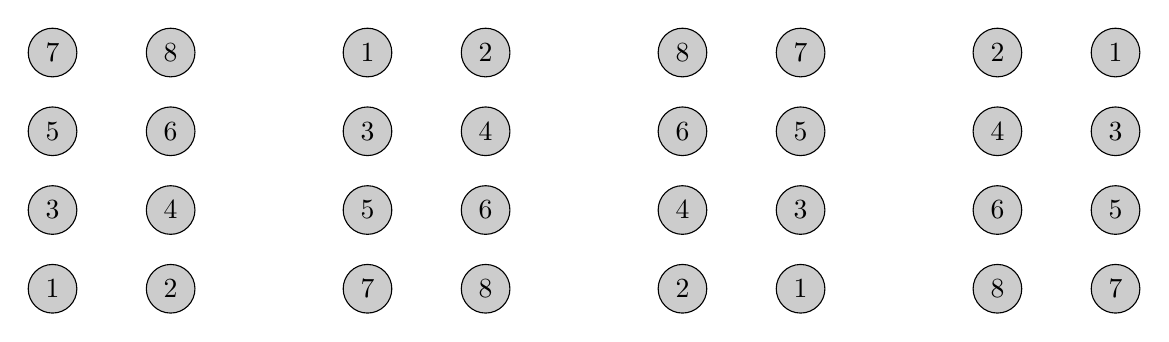
\begin{tikzpicture}
\begin{scope}
\node[circle,draw=black,fill=white!80!black,minimum size=3] (1) at (0,0)   {1};
\node[circle,draw=black,fill=white!80!black,minimum size=3] (2) at (1.5,0) {2};
\node[circle,draw=black,fill=white!80!black,minimum size=3] (3) at (0,1)   {3};
\node[circle,draw=black,fill=white!80!black,minimum size=3] (4) at (1.5,1) {4};
\node[circle,draw=black,fill=white!80!black,minimum size=3] (5) at (0,2)   {5};
\node[circle,draw=black,fill=white!80!black,minimum size=3] (6) at (1.5,2) {6};
\node[circle,draw=black,fill=white!80!black,minimum size=3] (7) at (0,3)   {7};
\node[circle,draw=black,fill=white!80!black,minimum size=3] (8) at (1.5,3) {8};
\end{scope}
\begin{scope}[shift={(4,0)}]
\node[circle,draw=black,fill=white!80!black,minimum size=3] (1) at (0,0)   {7};
\node[circle,draw=black,fill=white!80!black,minimum size=3] (2) at (1.5,0) {8};
\node[circle,draw=black,fill=white!80!black,minimum size=3] (3) at (0,1)   {5};
\node[circle,draw=black,fill=white!80!black,minimum size=3] (4) at (1.5,1) {6};
\node[circle,draw=black,fill=white!80!black,minimum size=3] (5) at (0,2)   {3};
\node[circle,draw=black,fill=white!80!black,minimum size=3] (6) at (1.5,2) {4};
\node[circle,draw=black,fill=white!80!black,minimum size=3] (7) at (0,3)   {1};
\node[circle,draw=black,fill=white!80!black,minimum size=3] (8) at (1.5,3) {2};
\end{scope}
\begin{scope}[shift={(8,0)}]
\node[circle,draw=black,fill=white!80!black,minimum size=3] (1) at (0,0)   {2};
\node[circle,draw=black,fill=white!80!black,minimum size=3] (2) at (1.5,0) {1};
\node[circle,draw=black,fill=white!80!black,minimum size=3] (3) at (0,1)   {4};
\node[circle,draw=black,fill=white!80!black,minimum size=3] (4) at (1.5,1) {3};
\node[circle,draw=black,fill=white!80!black,minimum size=3] (5) at (0,2)   {6};
\node[circle,draw=black,fill=white!80!black,minimum size=3] (6) at (1.5,2) {5};
\node[circle,draw=black,fill=white!80!black,minimum size=3] (7) at (0,3)   {8};
\node[circle,draw=black,fill=white!80!black,minimum size=3] (8) at (1.5,3) {7};
\end{scope}
\begin{scope}[shift={(12,0)}]
\node[circle,draw=black,fill=white!80!black,minimum size=3] (1) at (0,0)   {8};
\node[circle,draw=black,fill=white!80!black,minimum size=3] (2) at (1.5,0) {7};
\node[circle,draw=black,fill=white!80!black,minimum size=3] (3) at (0,1)   {6};
\node[circle,draw=black,fill=white!80!black,minimum size=3] (4) at (1.5,1) {5};
\node[circle,draw=black,fill=white!80!black,minimum size=3] (5) at (0,2)   {4};
\node[circle,draw=black,fill=white!80!black,minimum size=3] (6) at (1.5,2) {3};
\node[circle,draw=black,fill=white!80!black,minimum size=3] (7) at (0,3)   {2};
\node[circle,draw=black,fill=white!80!black,minimum size=3] (8) at (1.5,3) {1};
\end{scope}
\end{tikzpicture}
\caption{Arrangements obtained as solution for the HTC34 testbed}
\label{fig:arrangement}
\centering
\end{figure}

\section{WSU Tokyo testbed}
We evaluate our method using the WSU smart workplace testbed\cite{cook2010detection}, a publicly available data set. The testbed is located in a 12.2m $\times$ 10.9m  lab,  where students performed their normal work routine. The data was collected over a period of 4 months. 
The testbed consists of 43 motion sensors, placed as shown in the figure \ref{fig:casas}. The sensors field of view is $1.2m \times 1.2m$. In appendix \ref{app:wsuGrid} we provide a detailed explanation about how we obtain the grid adjacency matrix for the testbed.
First we choose a $4 \times 3$ grid which includes sensors 27, 22, 15, 28, 23, 16, 29, 24, 17, 30, 25, 18. This grid was chosen as it is mentioned in \cite{cook2010detection} that the region covered by these sensors is more active.
The data from the WSU testbed is represented in the form of a four tuple as shown in table \ref{tab:WSUDATA}. We re-sample the data at 100ms.

\begin{table}[]
\centering
\caption{Data structure of the WSU data.}
\label{tab:WSUDATA}
\begin{tabular}{|c|c|c|c|}
\hline
Date       & Time            & sensor & state \\ \hline
2008-01-02 & 08:02:19.58542  & M39    & ON    \\ \hline
2008-01-02 & 08:02:19.884461 & M41    & OFF   \\ \hline
2008-01-02 & 08:02:20.297468 & M32    & ON    \\ \hline
2008-01-02 & 08:02:20.297468 & M32    & ON    \\ \hline
2008-01-02 & 08:02:20.689425 & M31    & ON    \\ \hline
2008-01-02 & 08:02:21.957307 & M44    & OFF   \\ \hline
2008-01-02 & 08:02:22.517275 & M39    & OFF   \\ \hline
\end{tabular}
\end{table}

%We extract 10 dataset of 20 hrs each. Tes results obtained are as shown in the table \ref{tab:WSU4x3}

\begin{figure}
\includegraphics[scale=0.5]{./pics/LabSensorsLayout.jpg}
\centering
\caption{Floor plan for WSU CASAS office testbed, named Tokyo}
\label{fig:casas}
\end{figure}

\begin{figure}
\begin{subfigure}[b]{0.4\textwidth}
\includegraphics[scale=0.5]{./pics/corrTree.jpg}
\centering
\caption{Correaltion matrix $R$ represented as Graph $G$ with maximum spanning tree highlighted}
\label{fig:corrMatTree}
\end{subfigure}
\hfill
\begin{subfigure}[b]{0.4\textwidth}
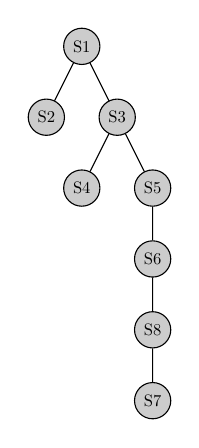
\begin{tikzpicture}[darkstyle/.style={circle,draw,fill=gray!40,minimum size=5,transform shape},scale=0.6]
\node[darkstyle]{S1}
	child{node[darkstyle]{S2}}
    child{node[darkstyle]{S3}
    	child{node[darkstyle]{S4}}
        child{node[darkstyle]{S5}
                child{node[darkstyle]{S6}
                child{node[darkstyle]{S8}
                child{node[darkstyle]{S7}}
                }}}};
\end{tikzpicture}
\caption{Maximum spanning tree of $R$}
\label{fig:corrMST}
\end{subfigure}
\end{figure}

%\[
%\begin{bmatrix}
%0&1&1&1&1&0&0&0\\
%1&0&1&1&0&1&0&0\\
%1&1&0&1&1&1&1&0\\
%1&1&1&0&1&1&0&1\\
%1&0&1&1&0&1&1&1\\
%0&1&1&1&1&0&1&1\\
%0&0&1&0&1&1&0&1\\
%0&0&0&1&1&1&1&0\\
%\end{bmatrix}
%\]
%
%\begin{figure}
%\begin{tikzpicture}
%\foreach \y[count=\xi] in {0,2.2}{
% \foreach \x [count=\yi] in {0,2.5,5,7.5}{
% 
% \ifthenelse{\xi=1}
% {
% \pgfmathtruncatemacro{\label}{(\yi-\xi)+\yi}
% }
% {
% \pgfmathtruncatemacro{\label}{\xi*\yi}
%}
% \node[circle,draw=black,fill=white!80!black,minimum size=5] (\label) at (\x,\y)  {\label} ;
% 
% 
%
%
%}
%}
%\draw (1)--(2) (1)--(3) (1)--(4) (2)--(3) (2)--(4) (3)--(4) (3)--(5) (5)--(7) (7)--(8)
%(6)--(8) (4)--(6) (6)--(5) (4)--(5) (6)--(3) (5)--(8) (6)--(7); 
%
%\draw (1)to[out=0-20,in=200](5);
%\draw (2)to[out=20,in=160](6);
%\draw (3)to[out=0-20,in=200](7);
%\draw (4)to[out=20,in=160](8);
%
%\end{tikzpicture}
%\centering
%\caption{Adjacency graph for the grid.}	
%\label{fig:adjGraph}
%\end{figure}




















\chapter{Conclusions and Future Work}
\label{chp:conclusionsandfuturework}

\section{Conclusions}
We present a new data driven method to identify the location of the sensors within a facility. We first identify a feature for the occupancy sensor data and calculate the correlation coefficient for the obtained feature data stream between the sensors. From the correlation values, we build correlation matrix ($R$)  which aids in identifying the neighboring sensor nodes. By computing the MST for $R$ we could identify at least one of the neighbors per sensor node. With the help of the coordinates of the vertices of the grid location, we model the grid as a graph and using the grid graph and the MST we reduce the problem of locating the sensors on the grid to a well-known problem of graph matching. We use the VF2 algorithm, a well known graph matching algorithm to map the sensor nodes to their locations on the grid. We validate the method developed with data from two different testbeds. We are able to identify the sensor locations with 0\% error for HTC testbed and $4\times3$ sub-layout grid for Tokyo testbed. For the entire layout of the Tokyo testbed, we were able to identify the location of all the 43 sensors except 3.  


\section{Future Work}
The results are encouraging, going forward we would like to address the following issues in the future:

\begin{itemize}
\item Determine the effect of overlapping region on the performance of the algorithm: As could be seen while evaluating the performance of our results with the Tokyo testbed, we could notice that the length of data required to obtain accurate results varied. One of the main factors could be the extent of overlap between the sensors. In the future, we would like to investigate the effect of overlapping region on the performance of our algorithm.
\item We are only able to identify the location of the sensors up to rotational symmetry. To overcome rotational symmetry and obtain the exact location of the sensors, extra information about the space is required. For our testbed, we can make use of the location of the door and observe the sensors which are triggered last before a large period of inactivity,this basically represents the last person leaving the room. The sensors which observe the last triggers can be placed on the side of the door and thus eliminating rotational symmetry in one direction. But this method cannot be generalized to all testbed. Therefore we would like to investigate methods which will be effective to eliminate the problem caused due to rotational symmetry.
\item Apply our approach to work with other sensors: In our work, we determine the location of the sensors using the correlation matrix obtained from the occupancy sensor data.
In the future, we would like to extend our method to other sensors. The modification that would have to be done to our approach would be to identify feature for the sensor data stream for which we can compute correlation values for the sensors. If we are able to obtain a correlation matrix such that the correlation values are high for neighboring sensors and low for non neighboring sensors, we could use our method to obtain the location of the sensors.
\item We have developed this method under the assumption that the grid is a connected graph, i.e every sensor has at least one neighboring sensor. In practice, it may not be the case that the grid will always be a connected graph, therefore we would like to expand our method such that it will be able to locate the sensors even when the grid is not a connected graph.
\end{itemize}


% BIBLIOGRAPHY
%#define SORTED 1
%\bibliographystyle{agsm}
\bibliography{./bib/mycollection}


\begin{appendix}

\chapter{HTC Testbed}
\label{app:A}
\section{Location information of the Grid}
\begin{wrapfigure}{r}{5.5cm}
\includegraphics[width=5.5cm]{./pics/angle.png}
\label{fig:height}
\end{wrapfigure}
The coordinates of the vertices are as given in the table \ref{tab:htc34xy}. We use EKMB1101112 PIR sensors from Panasonic, with detection angle of $82^\circ$.
PIR nodes are placed on the ceiling which is at a height of 3m. From this information we can compute the radius of the field of view of the PIR sensors as follows:\\\\
$h=3m, a = 82^{\circ}$\\
$r=h\cdot tan(\frac{a}{2})$\\
$r=2.6m$\\






\begin{table}[]
\centering
\caption{Coordinates of the vertices of the sensor network}
\label{tab:htc34xy}
\begin{tabular}{|c|c|c|}
\hline
vetrex & x   & y   \\ \hline
1      & 0   & 0   \\ \hline
2      & 0   & 2.2 \\ \hline
3      & 2.5 & 0   \\ \hline
4      & 2.5 & 2.2 \\ \hline
5      & 5   & 0   \\ \hline
6      & 5   & 2.2 \\ \hline
7      & 7.5 & 0   \\ \hline
8      & 7.5 & 2.2 \\ \hline
\end{tabular}
\end{table}

\begin{table}[]
\centering
\caption{Euclidean distances between vertices}
\label{tab:dist}
\begin{tabular}{|c|c|c|c|c|c|c|c|c|}
\hline
vertices & 1    & 2    & 3    & 4    & 5    & 6    & 7    & 8    \\ \hline
1        & 0.00 & 2.00 & 2.50 & 3.20 & 5.00 & 5.39 & 7.50 & 7.76 \\ \hline
2        & 2.00 & 0.00 & 3.20 & 2.50 & 5.39 & 5.00 & 7.76 & 7.50 \\ \hline
3        & 2.50 & 3.20 & 0.00 & 2.00 & 2.50 & 3.20 & 5.00 & 5.39 \\ \hline
4        & 3.20 & 2.50 & 2.00 & 0.00 & 3.20 & 2.50 & 5.39 & 5.00 \\ \hline
5        & 5.00 & 5.39 & 2.50 & 3.20 & 0.00 & 2.00 & 2.50 & 3.20 \\ \hline
6        & 5.39 & 5.00 & 3.20 & 2.50 & 2.00 & 0.00 & 3.20 & 2.50 \\ \hline
7        & 7.50 & 7.76 & 5.00 & 5.39 & 2.50 & 3.20 & 0.00 & 2.00 \\ \hline
8        & 7.76 & 7.50 & 5.39 & 5.00 & 3.20 & 2.50 & 2.00 & 0.00 \\ \hline
\end{tabular}
\end{table}

The distances between all the sensor nodes are represented in a matrix form and is as given in the table \ref{tab:dist} . The radius of the PIR sensor is 2.6m thus any 2 sensors located less than 5.2m(2r) apart are considered neighboring sensors. The adjacecy matrix is obtained as shown in the table \ref{tab:am}

\begin{table}[]
\centering
\caption{Adjacency matrix}
\label{tab:am}
\begin{tabular}{|c|c|c|c|c|c|c|c|c|}
\hline
vertices & 1 & 2 & 3 & 4 & 5 & 6 & 7 & 8 \\ \hline
1        & 0 & 1 & 1 & 1 & 1 & 0 & 0 & 0 \\ \hline
2        & 1 & 0 & 1 & 1 & 0 & 1 & 0 & 0 \\ \hline
3        & 1 & 1 & 0 & 1 & 1 & 1 & 1 & 0 \\ \hline
4        & 1 & 1 & 1 & 0 & 1 & 1 & 0 & 1 \\ \hline
5        & 1 & 0 & 1 & 1 & 0 & 1 & 1 & 1 \\ \hline
6        & 0 & 1 & 1 & 1 & 1 & 0 & 1 & 1 \\ \hline
7        & 0 & 0 & 1 & 0 & 1 & 1 & 0 & 1 \\ \hline
8        & 0 & 0 & 0 & 1 & 1 & 1 & 1 & 0 \\ \hline
\end{tabular}
\end{table}

\chapter{Tokyo Testbed}
\label{app:B}

The coordinates of the vertices in Tokyo testbed are not explicitly specified. The information available are the room layout map as shown in figure \ref{fig:casas}, pir sensor field of view given as $1.2m \times 1.2m$ and the average distance between the sensors as 1.2m in \cite{crandall2011tracking}. Assuming that the given layout is to scale and the distance between sensors 27 and 22 as 1.2m, the coordinates of all the sensors are computed. We start by placing the origin(0,0) at vertex 30 and measure the distance of every vertex from the x and y axis which gives the coordinates of all vertices on the grid. The coordinates thus obtained are as shown in the table \ref{tab:wsuxy}. No triggers was found for sensor 38 in the dataset, hence sensor 38 is not considered.

Adjacency between two vertices is determined if the square of dimension $1.2 \times 1.2$ drawn around the vertices have any overlap. If there is any overlap then the vertices are considered neighbors.


\begin{table}[]
\centering
\caption{Coordinates obtained for the vertices}
\label{tab:wsuxy}
\begin{tabular}{|c|c|c|c|c|c|c|c|c|c|c|c|}
\hline
vertices & x    & y     & vertices & x    & y     & vertices & x     & y     & vertices & x     & y     \\ \hline
1        & 4.40 & 5.60  & 12       & 3.60 & 0.00  & 23       & 1.20  & 2.00  & 34       & -0.60 & 5.00  \\ \hline
2        & 4.40 & 4.00  & 13       & 3.60 & -1.20 & 24       & 1.20  & 0.80  & 36       & -1.40 & 4.40  \\ \hline
3        & 4.40 & 3.20  & 14       & 2.40 & 3.60  & 25       & 1.20  & 0.00  & 37       & -1.80 & 4.80  \\ \hline
4        & 4.80 & 1.20  & 15       & 2.40 & 3.20  & 26       & 1.20  & -1.20 & 39       & -1.40 & -0.20 \\ \hline
5        & 4.80 & 0.00  & 16       & 2.40 & 2.00  & 27       & 0.00  & 3.20  & 40       & -2.20 & 1.88  \\ \hline
6        & 4.80 & -1.20 & 17       & 2.40 & 0.80  & 28       & 0.00  & 2.00  & 41       & -2.20 & 0.68  \\ \hline
7        & 3.40 & 5.60  & 18       & 2.40 & 0.00  & 29       & 0.00  & 0.80  & 42       & -2.20 & -0.52 \\ \hline
8        & 3.40 & 4.40  & 19       & 1.20 & 4.80  & 30       & 0.00  & 0.00  & 43       & -3.40 & 1.88  \\ \hline
9        & 3.40 & 3.20  & 20       & 0.60 & 4.64  & 31       & 0.00  & -1.20 & 44       & -3.40 & 0.68  \\ \hline
10       & 3.90 & 2.00  & 21       & 1.20 & 3.60  & 32       & -1.20 & -0.40 & 45       & -3.40 & -0.52 \\ \hline
11       & 3.60 & 1.20  & 22       & 1.20 & 3.20  & 33       & -0.60 & 3.80  &          &       &       \\ \hline
\end{tabular}
\end{table}











\end{appendix}

%\appendix

%\chapter{HTC Testbed}
\label{app:A}
\section{Location information of the Grid}
\begin{wrapfigure}{r}{5.5cm}
\includegraphics[width=5.5cm]{./pics/angle.png}
\label{fig:height}
\end{wrapfigure}
The coordinates of the vertices are as given in the table \ref{tab:htc34xy}. We use EKMB1101112 PIR sensors from Panasonic, with detection angle of $82^\circ$.
PIR nodes are placed on the ceiling which is at a height of 3m. From this information we can compute the radius of the field of view of the PIR sensors as follows:\\\\
$h=3m, a = 82^{\circ}$\\
$r=h\cdot tan(\frac{a}{2})$\\
$r=2.6m$\\






\begin{table}[]
\centering
\caption{Coordinates of the vertices of the sensor network}
\label{tab:htc34xy}
\begin{tabular}{|c|c|c|}
\hline
vetrex & x   & y   \\ \hline
1      & 0   & 0   \\ \hline
2      & 0   & 2.2 \\ \hline
3      & 2.5 & 0   \\ \hline
4      & 2.5 & 2.2 \\ \hline
5      & 5   & 0   \\ \hline
6      & 5   & 2.2 \\ \hline
7      & 7.5 & 0   \\ \hline
8      & 7.5 & 2.2 \\ \hline
\end{tabular}
\end{table}

\begin{table}[]
\centering
\caption{Euclidean distances between vertices}
\label{tab:dist}
\begin{tabular}{|c|c|c|c|c|c|c|c|c|}
\hline
vertices & 1    & 2    & 3    & 4    & 5    & 6    & 7    & 8    \\ \hline
1        & 0.00 & 2.00 & 2.50 & 3.20 & 5.00 & 5.39 & 7.50 & 7.76 \\ \hline
2        & 2.00 & 0.00 & 3.20 & 2.50 & 5.39 & 5.00 & 7.76 & 7.50 \\ \hline
3        & 2.50 & 3.20 & 0.00 & 2.00 & 2.50 & 3.20 & 5.00 & 5.39 \\ \hline
4        & 3.20 & 2.50 & 2.00 & 0.00 & 3.20 & 2.50 & 5.39 & 5.00 \\ \hline
5        & 5.00 & 5.39 & 2.50 & 3.20 & 0.00 & 2.00 & 2.50 & 3.20 \\ \hline
6        & 5.39 & 5.00 & 3.20 & 2.50 & 2.00 & 0.00 & 3.20 & 2.50 \\ \hline
7        & 7.50 & 7.76 & 5.00 & 5.39 & 2.50 & 3.20 & 0.00 & 2.00 \\ \hline
8        & 7.76 & 7.50 & 5.39 & 5.00 & 3.20 & 2.50 & 2.00 & 0.00 \\ \hline
\end{tabular}
\end{table}

The distances between all the sensor nodes are represented in a matrix form and is as given in the table \ref{tab:dist} . The radius of the PIR sensor is 2.6m thus any 2 sensors located less than 5.2m(2r) apart are considered neighboring sensors. The adjacecy matrix is obtained as shown in the table \ref{tab:am}

\begin{table}[]
\centering
\caption{Adjacency matrix}
\label{tab:am}
\begin{tabular}{|c|c|c|c|c|c|c|c|c|}
\hline
vertices & 1 & 2 & 3 & 4 & 5 & 6 & 7 & 8 \\ \hline
1        & 0 & 1 & 1 & 1 & 1 & 0 & 0 & 0 \\ \hline
2        & 1 & 0 & 1 & 1 & 0 & 1 & 0 & 0 \\ \hline
3        & 1 & 1 & 0 & 1 & 1 & 1 & 1 & 0 \\ \hline
4        & 1 & 1 & 1 & 0 & 1 & 1 & 0 & 1 \\ \hline
5        & 1 & 0 & 1 & 1 & 0 & 1 & 1 & 1 \\ \hline
6        & 0 & 1 & 1 & 1 & 1 & 0 & 1 & 1 \\ \hline
7        & 0 & 0 & 1 & 0 & 1 & 1 & 0 & 1 \\ \hline
8        & 0 & 0 & 0 & 1 & 1 & 1 & 1 & 0 \\ \hline
\end{tabular}
\end{table}

\chapter{Tokyo Testbed}
\label{app:B}

The coordinates of the vertices in Tokyo testbed are not explicitly specified. The information available are the room layout map as shown in figure \ref{fig:casas}, pir sensor field of view given as $1.2m \times 1.2m$ and the average distance between the sensors as 1.2m in \cite{crandall2011tracking}. Assuming that the given layout is to scale and the distance between sensors 27 and 22 as 1.2m, the coordinates of all the sensors are computed. We start by placing the origin(0,0) at vertex 30 and measure the distance of every vertex from the x and y axis which gives the coordinates of all vertices on the grid. The coordinates thus obtained are as shown in the table \ref{tab:wsuxy}. No triggers was found for sensor 38 in the dataset, hence sensor 38 is not considered.

Adjacency between two vertices is determined if the square of dimension $1.2 \times 1.2$ drawn around the vertices have any overlap. If there is any overlap then the vertices are considered neighbors.


\begin{table}[]
\centering
\caption{Coordinates obtained for the vertices}
\label{tab:wsuxy}
\begin{tabular}{|c|c|c|c|c|c|c|c|c|c|c|c|}
\hline
vertices & x    & y     & vertices & x    & y     & vertices & x     & y     & vertices & x     & y     \\ \hline
1        & 4.40 & 5.60  & 12       & 3.60 & 0.00  & 23       & 1.20  & 2.00  & 34       & -0.60 & 5.00  \\ \hline
2        & 4.40 & 4.00  & 13       & 3.60 & -1.20 & 24       & 1.20  & 0.80  & 36       & -1.40 & 4.40  \\ \hline
3        & 4.40 & 3.20  & 14       & 2.40 & 3.60  & 25       & 1.20  & 0.00  & 37       & -1.80 & 4.80  \\ \hline
4        & 4.80 & 1.20  & 15       & 2.40 & 3.20  & 26       & 1.20  & -1.20 & 39       & -1.40 & -0.20 \\ \hline
5        & 4.80 & 0.00  & 16       & 2.40 & 2.00  & 27       & 0.00  & 3.20  & 40       & -2.20 & 1.88  \\ \hline
6        & 4.80 & -1.20 & 17       & 2.40 & 0.80  & 28       & 0.00  & 2.00  & 41       & -2.20 & 0.68  \\ \hline
7        & 3.40 & 5.60  & 18       & 2.40 & 0.00  & 29       & 0.00  & 0.80  & 42       & -2.20 & -0.52 \\ \hline
8        & 3.40 & 4.40  & 19       & 1.20 & 4.80  & 30       & 0.00  & 0.00  & 43       & -3.40 & 1.88  \\ \hline
9        & 3.40 & 3.20  & 20       & 0.60 & 4.64  & 31       & 0.00  & -1.20 & 44       & -3.40 & 0.68  \\ \hline
10       & 3.90 & 2.00  & 21       & 1.20 & 3.60  & 32       & -1.20 & -0.40 & 45       & -3.40 & -0.52 \\ \hline
11       & 3.60 & 1.20  & 22       & 1.20 & 3.20  & 33       & -0.60 & 3.80  &          &       &       \\ \hline
\end{tabular}
\end{table}











\end{document}
